% !TeX program = xelatex
% !TeX encoding = UTF-8
\documentclass[sigconf,nonacm]{acmart}

\usepackage{xeCJK}
\setCJKmainfont{SimSun}
\usepackage{booktabs}
\usepackage{graphicx}
\usepackage{amsmath}
\usepackage{array}
\usepackage{float}

\AtBeginDocument{%
  \providecommand\BibTeX{{Bib\TeX}}%
}
\settopmatter{printacmref=false}
\renewcommand\footnotetextcopyrightpermission[1]{}
\pagestyle{plain}

\title{AIGC 图像的频谱指纹挖掘与伪造检测}
\author{Team members: [fill in]}
\affiliation{%
  \institution{[fill in]}
  \city{[fill in]}
  \country{China}
}
\email{[fill in]}

\begin{document}

\begin{abstract}
本文面向课程第五题，研究 AIGC 图像在频率域中的可检测指纹。我们使用 GenImage 中 ADM、BigGAN、VQDM 和 GLIDE 四个生成源，构建两个任务：AI/真实图像二分类，以及 AI 图像生成源归因。方法不依赖 CNN 或 Vision Transformer，而是提取 FFT、DCT、颜色频谱、多尺度频谱、块 DCT 与残差频谱统计，并使用 LightGBM 完成浅层可解释建模。最终主模型为 \texttt{fusion\_freq + flat LightGBM + wide profile}，在 full 训练比例下达到二分类 macro-F1 0.9913、AUC 0.9996，归因 macro-F1 0.9991，双任务平均 macro-F1 0.9952。进一步实验表明：频谱融合特征在 clean validation 上极强，但在 JPEG、缩放和高斯噪声等 degraded 场景下明显退化；跨生成器留一测试也显示模型仍会学习到特定生成器的指纹。该结果说明频谱指纹能够有效检测 AIGC 图像，同时鲁棒性与跨生成器泛化仍是关键限制。
\end{abstract}

\maketitle

\section{Introduction}
扩散模型和 GAN 生成图像的视觉质量持续提升，单靠肉眼已经难以稳定判断图像来源。课程题目要求从像素空间转向频率空间，挖掘人眼不可见但可统计建模的 AIGC 数字指纹。本文因此不把重点放在语义内容识别，而是研究生成过程、上采样链路、压缩后处理和噪声分布可能残留在频谱中的结构化痕迹。

本文围绕三个问题展开：RQ1，FFT/DCT 等频谱统计能否区分 AI 图像与真实图像；RQ2，频谱特征能否识别生成源；RQ3，JPEG、缩放和噪声扰动会怎样破坏或保留频谱指纹。我们的贡献包括：构建四生成源 GenImage 频谱检测流程；比较 baseline、调参、scale-up 和频域增强路线；加入跨生成器泛化、鲁棒性诊断、置信度拒识和错误模式分析；最终形成一个轻量、可解释、可复现的 AIGC 检测闭环。

\section{Dataset and Protocol}
本文使用 GenImage 数据集~\cite{zhu2023genimage} 中四个生成源子集：ADM、BigGAN、VQDM 和 GLIDE。数据根目录为 \texttt{C:\textbackslash Users\textbackslash 99303\textbackslash git\textbackslash GenImage\_data}。每个生成源都包含 \texttt{train/ai}、\texttt{train/nature}、\texttt{val/ai} 和 \texttt{val/nature}。实验中 \texttt{train} 用于训练，\texttt{val} 作为测试集。

二分类任务合并四个生成源下的 AI 与 nature 图像，标签为 \texttt{ai} 和 \texttt{nature}。归因任务只使用 AI 图像，标签为 ADM、BigGAN、VQDM 和 GLIDE。抽样实验均使用分层采样和固定 seed；最终主结果使用 full 训练比例。鲁棒性评估不参与训练，只在同一个 20\% validation 子集上施加 JPEG、resize 和 Gaussian noise。

\begin{table}[H]
  \centering
  \caption{GenImage 四个生成源的本地数据规模。}
  \label{tab:dataset-counts}
  \begin{tabular}{lrrrr}
    \toprule
    Generator & Train AI & Train Nature & Val AI & Val Nature \\
    \midrule
    ADM & 162000 & 157453 & 6000 & 6000 \\
    BigGAN & 162000 & 162000 & 6000 & 6000 \\
    VQDM & 162000 & 162000 & 6000 & 6000 \\
    GLIDE & 162000 & 162000 & 6000 & 6000 \\
    \bottomrule
  \end{tabular}
\end{table}

\section{Method}
基础流程首先将图像 resize 到 $256\times256$，对灰度图去均值并施加 Hann 窗，然后计算二维 FFT 功率谱：
\[
P(u,v)=\log(1+|\mathcal{F}(I)(u,v)|^2).
\]
baseline 特征包括 FFT 径向功率谱、角向能量、低/中/高频能量比例、频谱斜率、高频残差统计、patch 级高频变化和 DCT 径向谱。为进一步提分，本文实现 \texttt{fusion\_freq} profile：在 RGB 与 YCbCr 通道上提取颜色频谱，在 $128/256/384$ 三个尺度上提取多尺度频谱，加入 8x8 block-DCT AC 能量和块边界统计，并对高通、median 与 Laplacian 残差再做频谱统计。所有特征都对应明确的信号处理统计，不依赖语义表征。

这些频域特征的设计目标不是简单增加维度，而是覆盖生成图像可能留下指纹的几个互补来源。第一，径向功率谱和频谱斜率描述自然图像常见的能量衰减规律。如果生成模型的上采样、去噪或后处理链路改变了高低频能量分配，径向统计会直接反映这种偏移。第二，角向能量与块 DCT 统计用于捕获方向性纹理和局部周期结构。真实相机图像中的纹理方向通常与场景内容相关，而生成模型可能产生更规则的方向性伪影；JPEG-like 块边界也会改变局部 DCT AC 能量。第三，颜色频谱把灰度空间中被平均掉的通道差异重新引入模型。扩散模型和 GAN 在 RGB 或 YCbCr 通道上可能具有不同的高频噪声分布，因此颜色频域特征在第二轮实验中贡献最大。第四，残差频谱弱化低频语义轮廓，突出高通、median 和 Laplacian 残差中的细粒度噪声。该组特征有助于区分自然图像的传感器噪声与生成图像的合成残差。

本文同时保留了“单一频域”和“融合频域”两套实验口径。单一频域实验用于回答某一类信号是否独立有效，例如只用颜色频谱或只用 block-DCT 是否已经能完成检测；融合频域实验则用于回答这些信号是否互补。这样做可以避免把提升简单归因于特征数量增加。若某个单一 profile 已经接近融合 profile，则说明主要信息集中在该频域；若多个单一 profile 都弱于融合 profile，则说明不同频域捕获了不同类型的生成痕迹。后续结果显示颜色频谱最强，但融合频域仍进一步提升，因此最终方法采用 \texttt{fusion\_freq} 作为主路线。

监督模型以 LightGBM~\cite{ke2017lightgbm} 为主，RandomForest 和 LogisticRegression 作为早期 baseline。最终路线使用 flat LightGBM、多分类归因、\texttt{wide} 参数 profile 和二分类阈值校准。LightGBM 训练优先使用 GPU；若 GPU 在复杂多分类训练中失败，代码自动 fallback 到 CPU。频谱特征提取主要依赖 CPU 多进程和 feature cache。信号处理背景参考 Oppenheim 等人的经典教材~\cite{oppenheim1999discrete}。

选择 LightGBM 的原因有三点。首先，它能处理数百到上千维手工统计特征，并给出稳定的 feature importance，因此适合课程要求中的“可解释模型”。其次，它比深度 CNN/ViT 更容易复现，训练结果主要受特征和抽样策略影响，而不是受大量超参数或预训练权重影响。第三，树模型可以较自然地建模频带比值、颜色通道能量和残差统计之间的非线性组合。为了控制过拟合，本文没有把所有中间实验都作为最终结论，而是使用 5\% 调参、10\% 验证、20/50/full scale-up 的逐级流程来确认提升是否稳定。

\section{Experiments}
实验分为五层。第一层使用 1\%、5\% 和 10\% 抽样验证原始 FFT/DCT baseline，并完成 LightGBM 调参。第二层进行 20\%、50\% 和 full scale-up，确认样本量扩大能稳定提升 clean performance。第三层进行频域增强，比较 \texttt{color\_freq}、\texttt{multiscale\_freq}、\texttt{block\_dct}、\texttt{residual\_freq} 和 \texttt{fusion\_freq}。第四层固定最终模型，在 validation 图像上施加 JPEG、resize 和 Gaussian noise，诊断后处理扰动下的失效模式。第五层扩展分析跨生成器泛化、鲁棒训练、稳健频谱 profile 和置信度拒识。

所有主要结果通过 \texttt{metrics\_summary.json}、\texttt{model\_comparison.csv}、混淆矩阵、feature importance、robustness CSV 和 confidence CSV 自动汇总到 \texttt{report/tables} 与 \texttt{report/figures}。Notebook 只读取这些资产，不重新执行大规模训练。

工程实现上，实验被拆分为可中断、可恢复的输出目录。每个任务目录都保存模型比较表、最佳模型、混淆矩阵、错误样本和配置文件；特征缓存单独存放，避免重复扫描完整图像集。这样做的意义在于：一方面，full-scale 频谱特征提取耗时较长，缓存能保证后续调参、鲁棒性评估和 Notebook 展示不必重复计算；另一方面，不同阶段的输出目录天然形成实验记录，报告中的每张图都可以追溯到具体 CSV 或 JSON。对于队友分机器运行得到的结果，本文也只把最终 CSV/PNG 资产纳入报告，不把数据集、缓存和大模型输出提交到仓库。

评价指标以 macro-F1 为主，因为二分类与归因任务都需要避免被某个类别的大样本量掩盖。二分类同时记录 AUC，用于观察阈值之外的排序能力；归因任务主要关注混淆矩阵，尤其是 ADM 与 VQDM 之间的系统性错误。鲁棒性部分不只看 clean 分数，还统计每种扰动级别下的 macro-F1、预测分布和 degraded 平均 F1。跨生成器泛化实验只训练二分类器，因为它更直接回答“是否学到通用 AIGC 指纹”，而不是在未见生成源标签不存在时强行做归因。

\section{Results and Analysis}
\subsection{Clean Performance}
表~\ref{tab:main-results} 汇总了从旧灰度 baseline 到第二轮频域融合优化的关键结果。第一轮 full baseline 的双任务平均 macro-F1 为 0.9042；引入 \texttt{fusion\_freq} 后，5\% 抽样已经达到 0.9919，full 训练比例进一步达到 0.9952。最终主结果固定为 \texttt{outputs\_v2\_full\_best}，不把后续鲁棒训练分支替代为主模型。

\begin{table}[H]
  \centering
  \caption{主要 clean 结果对比。}
  \label{tab:main-results}
  \begin{tabular}{llrrr}
    \toprule
    Run & Feature & Binary F1 & Attr. F1 & Avg. F1 \\
    \midrule
    gray full baseline & FFT/DCT & 0.8997 & 0.9086 & 0.9042 \\
    v2 5\% flat & fusion & 0.9871 & 0.9967 & 0.9919 \\
    v2 20\% flat & fusion & 0.9910 & 0.9973 & 0.9942 \\
    v2 50\% flat & fusion & 0.9911 & 0.9984 & 0.9948 \\
    v2 full best & fusion & \textbf{0.9913} & \textbf{0.9991} & \textbf{0.9952} \\
    \bottomrule
  \end{tabular}
\end{table}

\begin{figure}[H]
  \centering
  \IfFileExists{figures/optimization_v2_macro_f1.png}{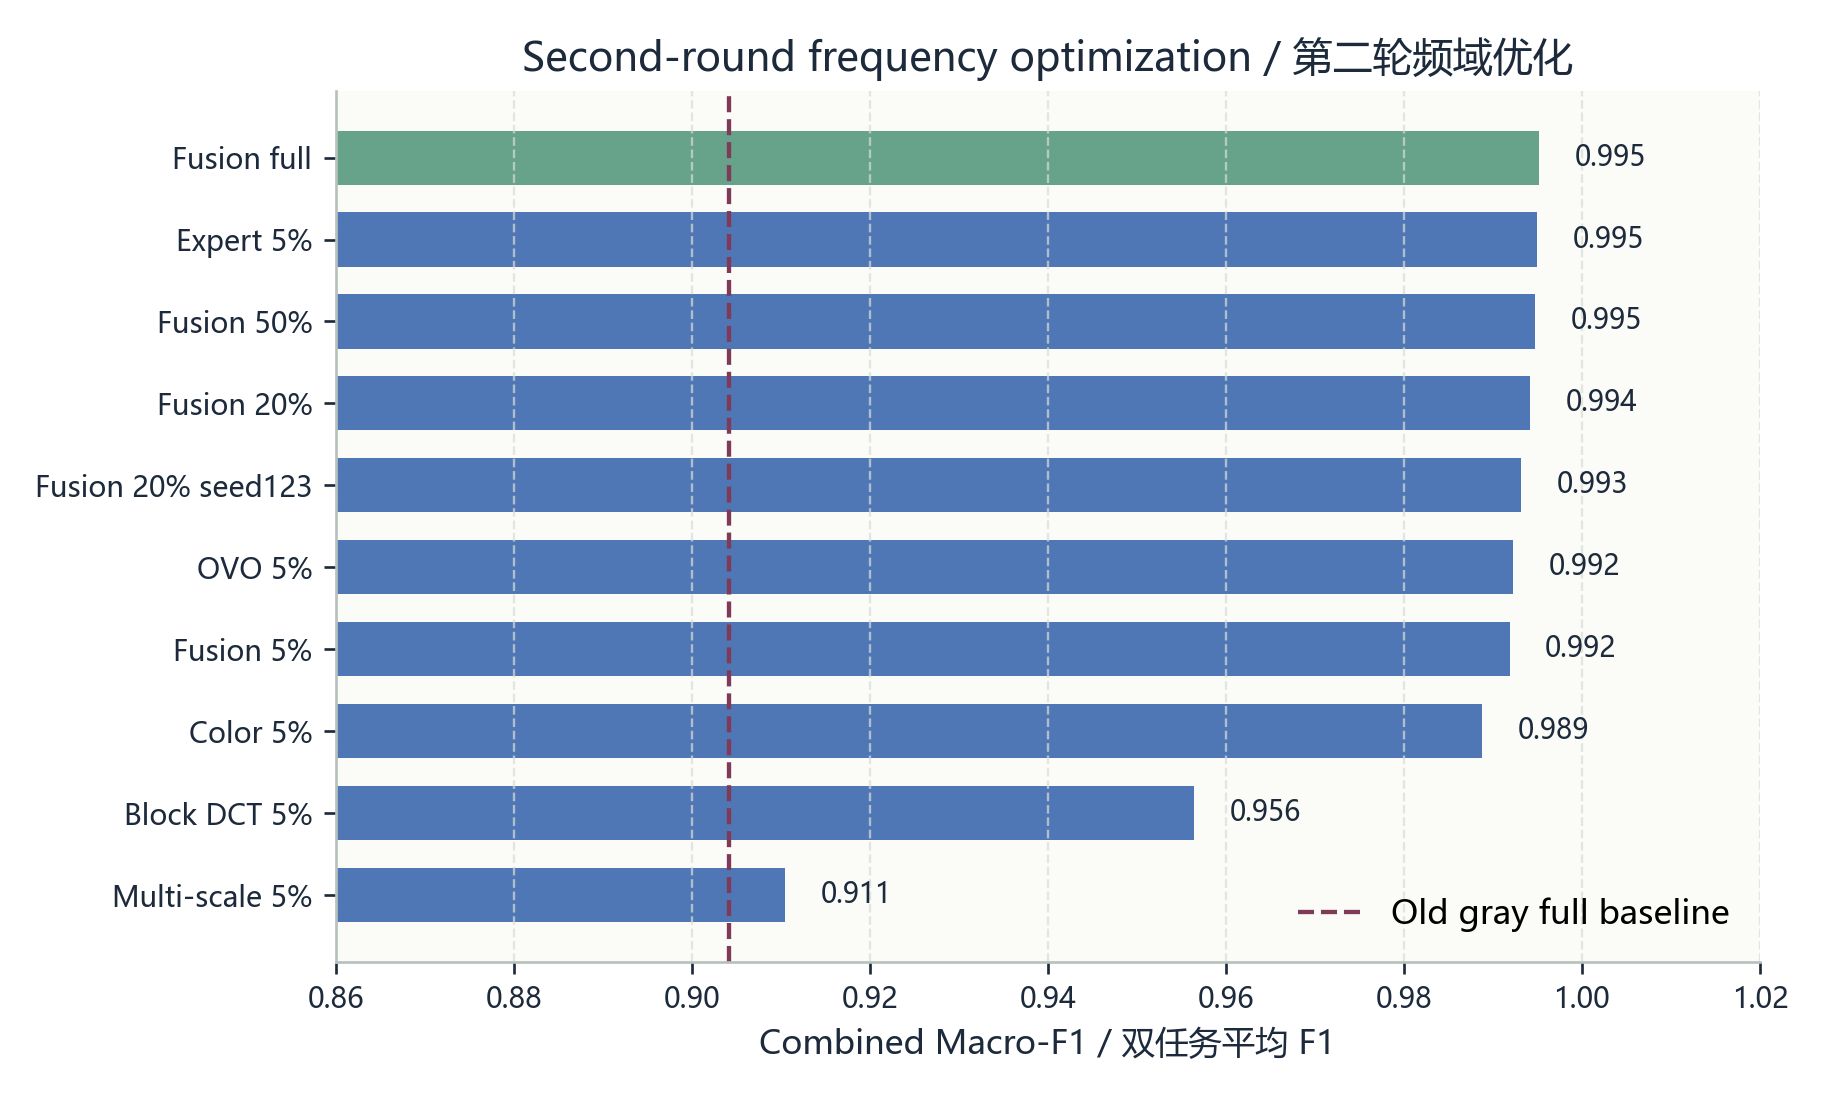
\includegraphics[width=0.49\linewidth]{figures/optimization_v2_macro_f1.png}}{\fbox{missing}}
  \IfFileExists{figures/scaleup_macro_f1.png}{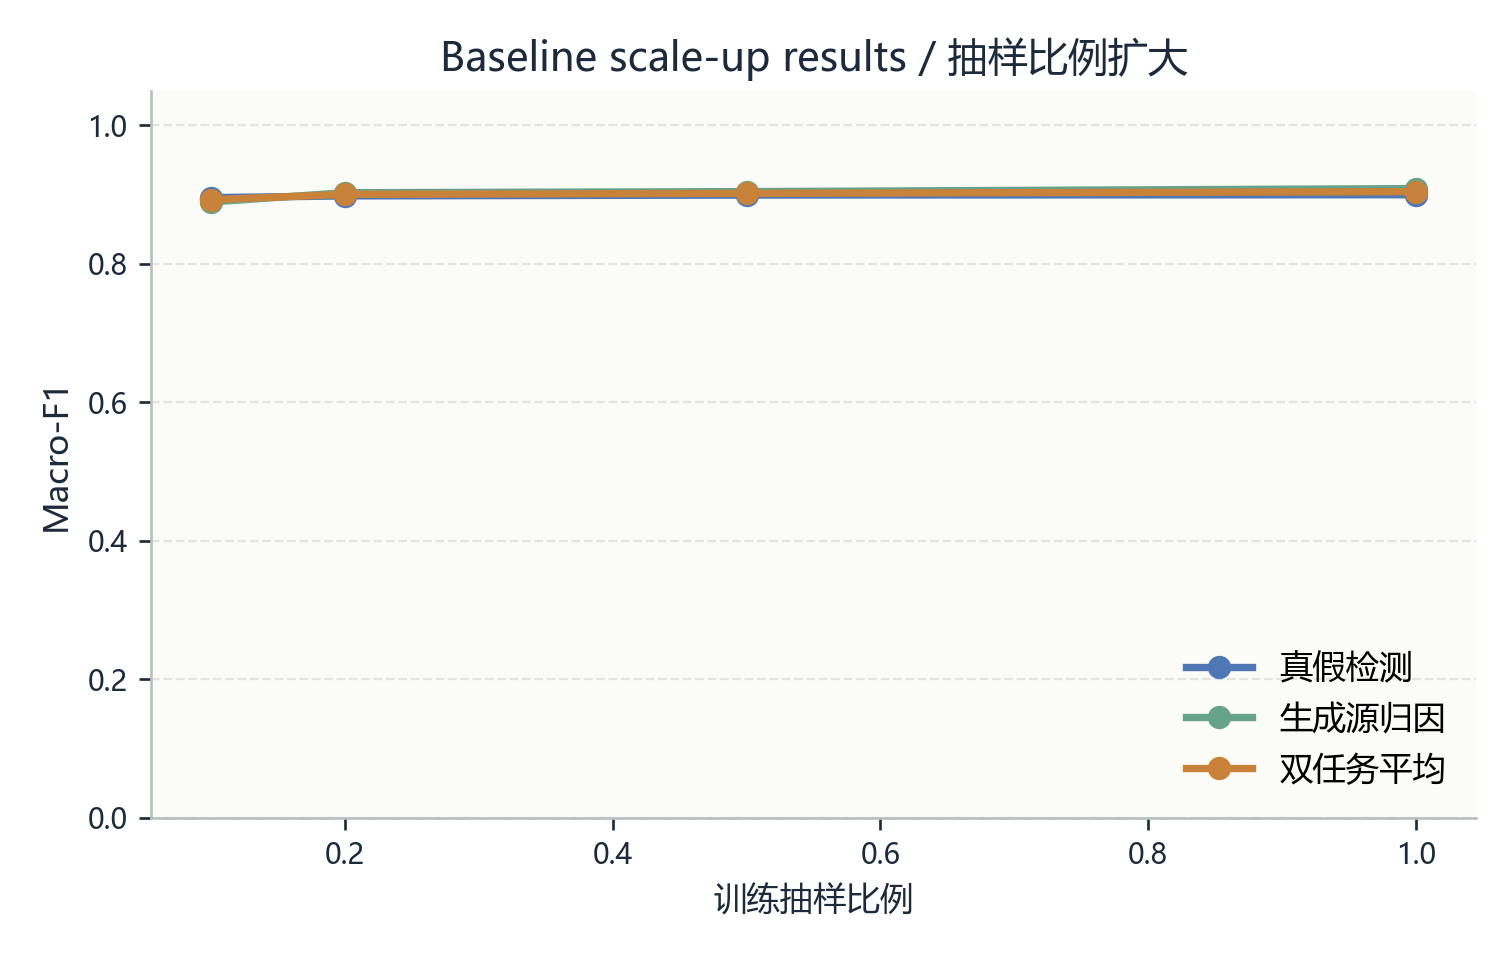
\includegraphics[width=0.49\linewidth]{figures/scaleup_macro_f1.png}}{\fbox{missing}}
  \caption{第二轮频域优化和抽样比例扩大带来的 clean performance 提升。}
  \label{fig:optimization-scale}
\end{figure}

\subsection{Single-Domain and Fused Frequency Results}
为了区分“单一频域特征有效”与“融合频域特征更强”这两个结论，本文将第二轮特征实验拆成两类。第一类是单一或局部频域 profile：\texttt{color\_freq} 只强调 RGB/YCbCr 颜色通道频谱，\texttt{multiscale\_freq} 只强调不同 resize 尺度的功率谱，\texttt{block\_dct} 关注局部 8x8 DCT 与 JPEG-like 块结构，\texttt{residual\_freq} 关注高通、median 和 Laplacian 残差频谱。第二类是 \texttt{fusion\_freq}，它将颜色、多尺度、块 DCT 和残差频谱合并到同一个特征向量中。

图~\ref{fig:single-fusion} 给出了单一频域与融合频域 profile 的直接对比。在相同 5\% 抽样下，\texttt{color\_freq} 的双任务平均 F1 约为 0.9887，是最强的单一频域 profile；\texttt{block\_dct}、\texttt{multiscale\_freq} 和 \texttt{residual\_freq} 单独使用时均明显弱于颜色频谱。融合频域在 5\% 抽样下已经达到 0.9919，full scale 后进一步达到 0.9952。这个结果说明单一频域确实含有 AIGC 指纹，但不同频域统计之间存在互补性：颜色频谱提供强判别信号，多尺度和块 DCT 描述采样/压缩痕迹，残差频谱补充局部生成噪声差异。

\begin{figure}[H]
  \centering
  \IfFileExists{figures/single_vs_fusion_feature_profiles.png}{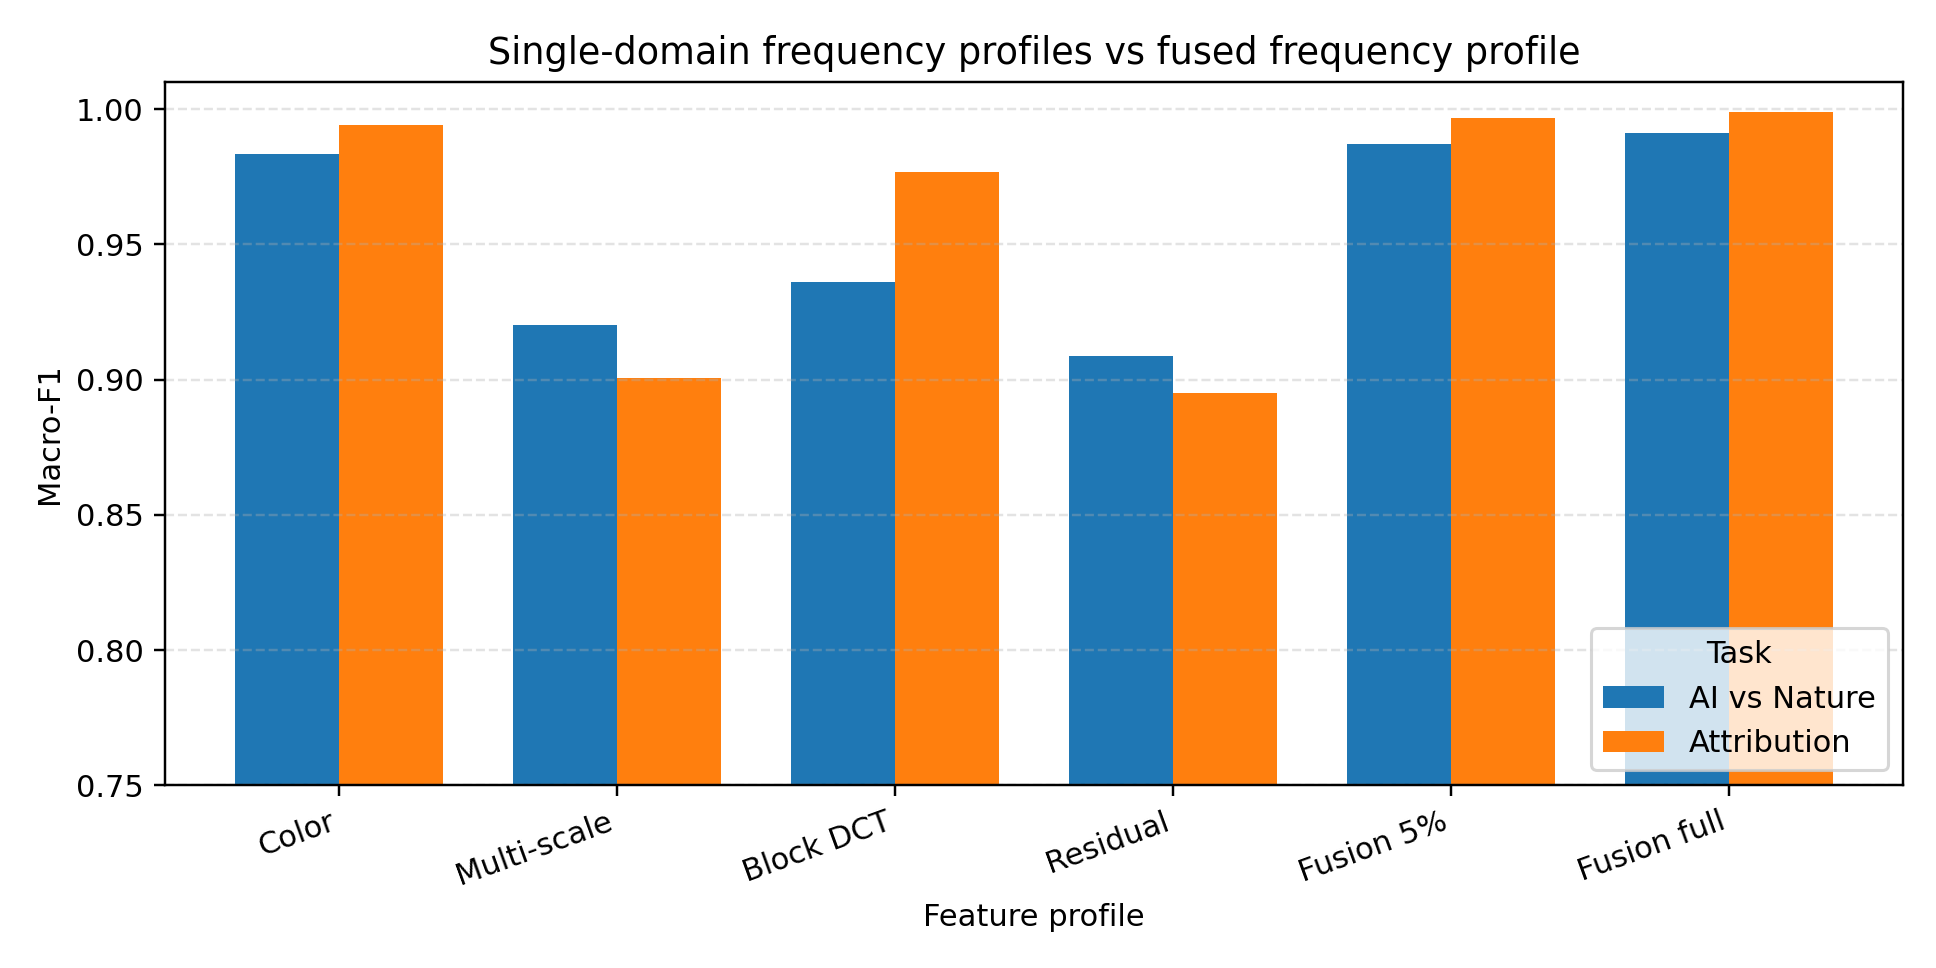
\includegraphics[width=\linewidth]{figures/single_vs_fusion_feature_profiles.png}}{\fbox{missing}}
  \caption{单一频域 profile 与融合频域 profile 的实验结果。单一频域包括颜色频谱、多尺度频谱、块 DCT 和残差频谱；融合频域将这些信号合并后在 5\% 与 full 设置下都取得更高 F1。}
  \label{fig:single-fusion}
\end{figure}

进一步的 feature ablation 结果见图~\ref{fig:ablation-single}。在早期灰度 FFT/DCT baseline 中，\texttt{fft\_radial} 与 \texttt{no\_dct} 表现最强，说明径向功率谱已经能捕获大量真假差异；\texttt{patch\_high\_freq} 单独使用最弱，说明局部高频变化不足以单独支撑稳定检测。归因任务中也出现类似排序，表明生成源差异主要分布在全局频谱形态，而不是单一局部纹理统计。该消融图补充说明：融合频域不是简单堆叠无关特征，而是在多个有独立贡献的频谱视角上进行组合。

\begin{figure}[H]
  \centering
  \IfFileExists{figures/feature_ablation_binary_ai_vs_nature.png}{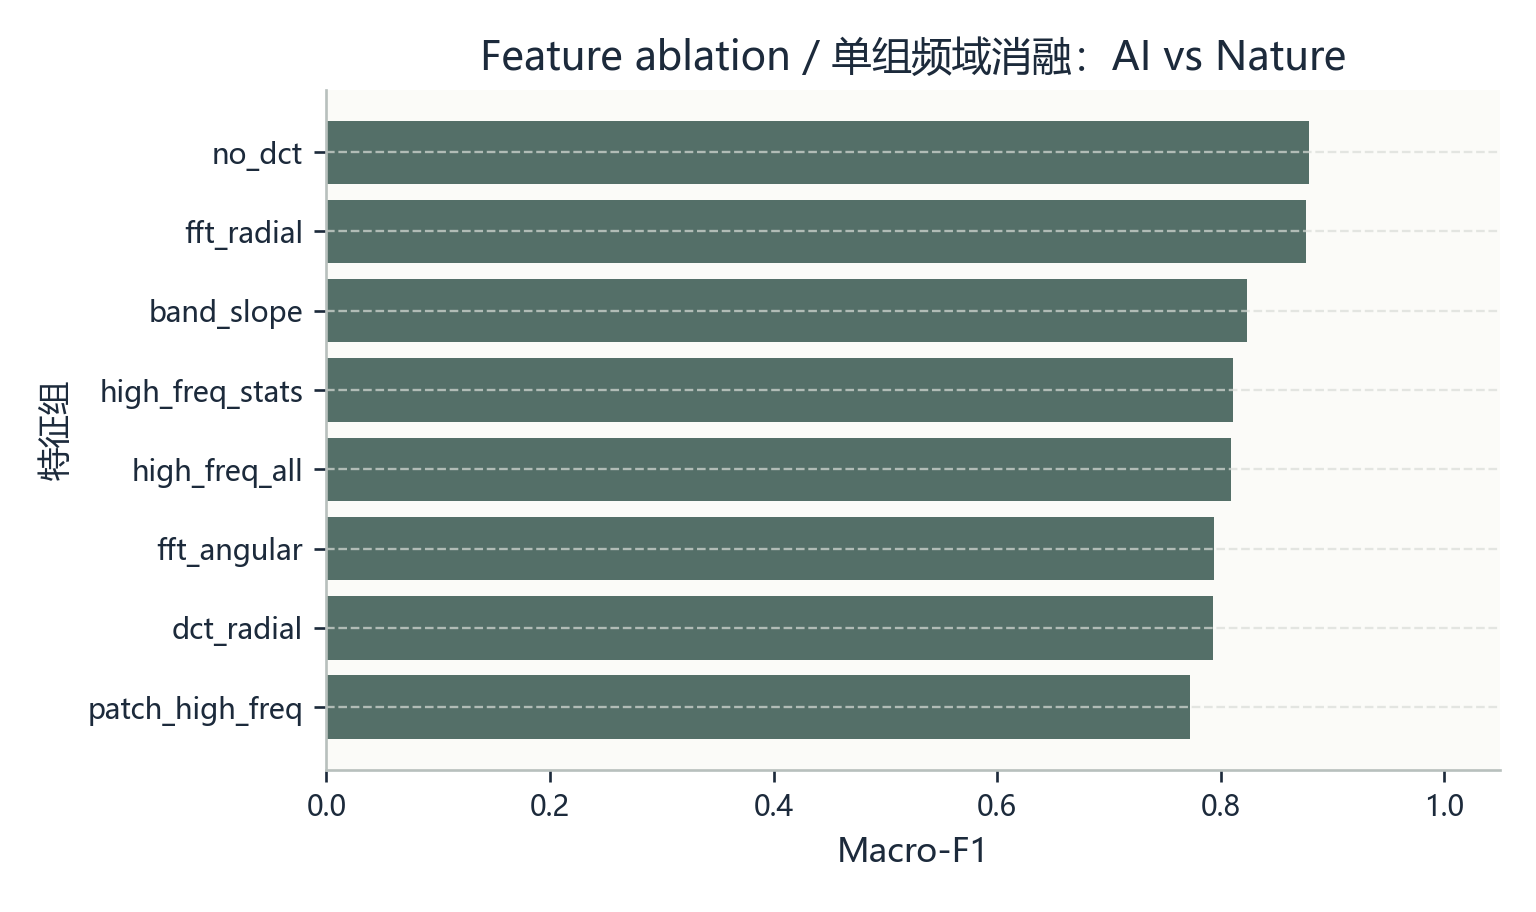
\includegraphics[width=0.49\linewidth]{figures/feature_ablation_binary_ai_vs_nature.png}}{\fbox{missing}}
  \IfFileExists{figures/feature_ablation_ai_subsource_attribution.png}{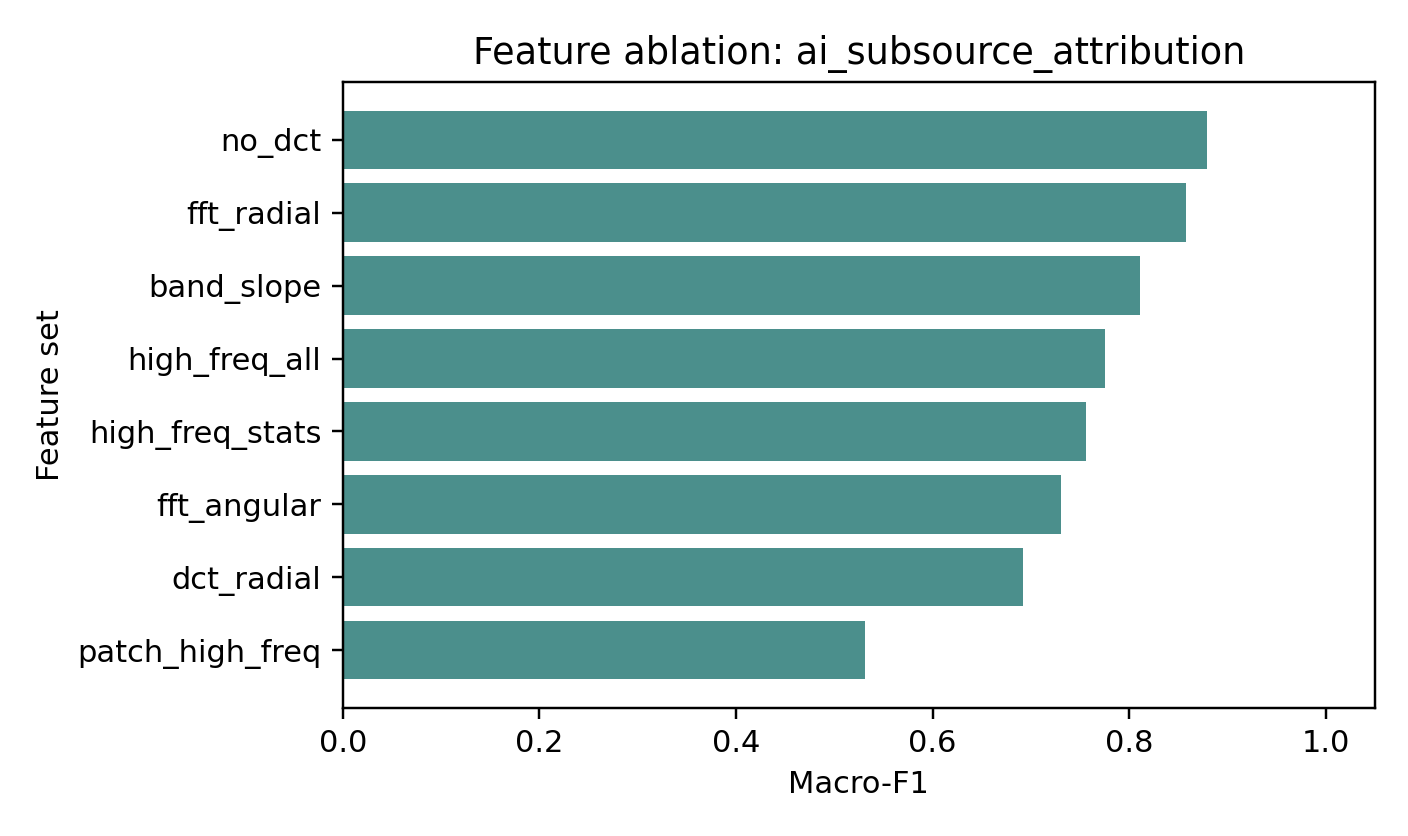
\includegraphics[width=0.49\linewidth]{figures/feature_ablation_ai_subsource_attribution.png}}{\fbox{missing}}
  \caption{单一频域/单组频谱特征的消融实验结果。左图为真假二分类，右图为生成源归因；径向功率谱和频带斜率贡献稳定，局部 patch 高频特征单独使用时较弱。}
  \label{fig:ablation-single}
\end{figure}

图~\ref{fig:spectrum-examples} 展示了从原图到频谱图的可视化示例。真实图像通常具有更接近自然图像统计的径向能量衰减，而生成图像可能在高频区域、颜色通道或局部残差中出现结构化偏置。虽然单张图不能直接证明模型决策，但这种可视化能帮助解释为什么浅层频谱统计可以在不理解语义内容的情况下区分 AIGC 图像。

\begin{figure}[H]
  \centering
  \IfFileExists{figures/spectrum_examples.png}{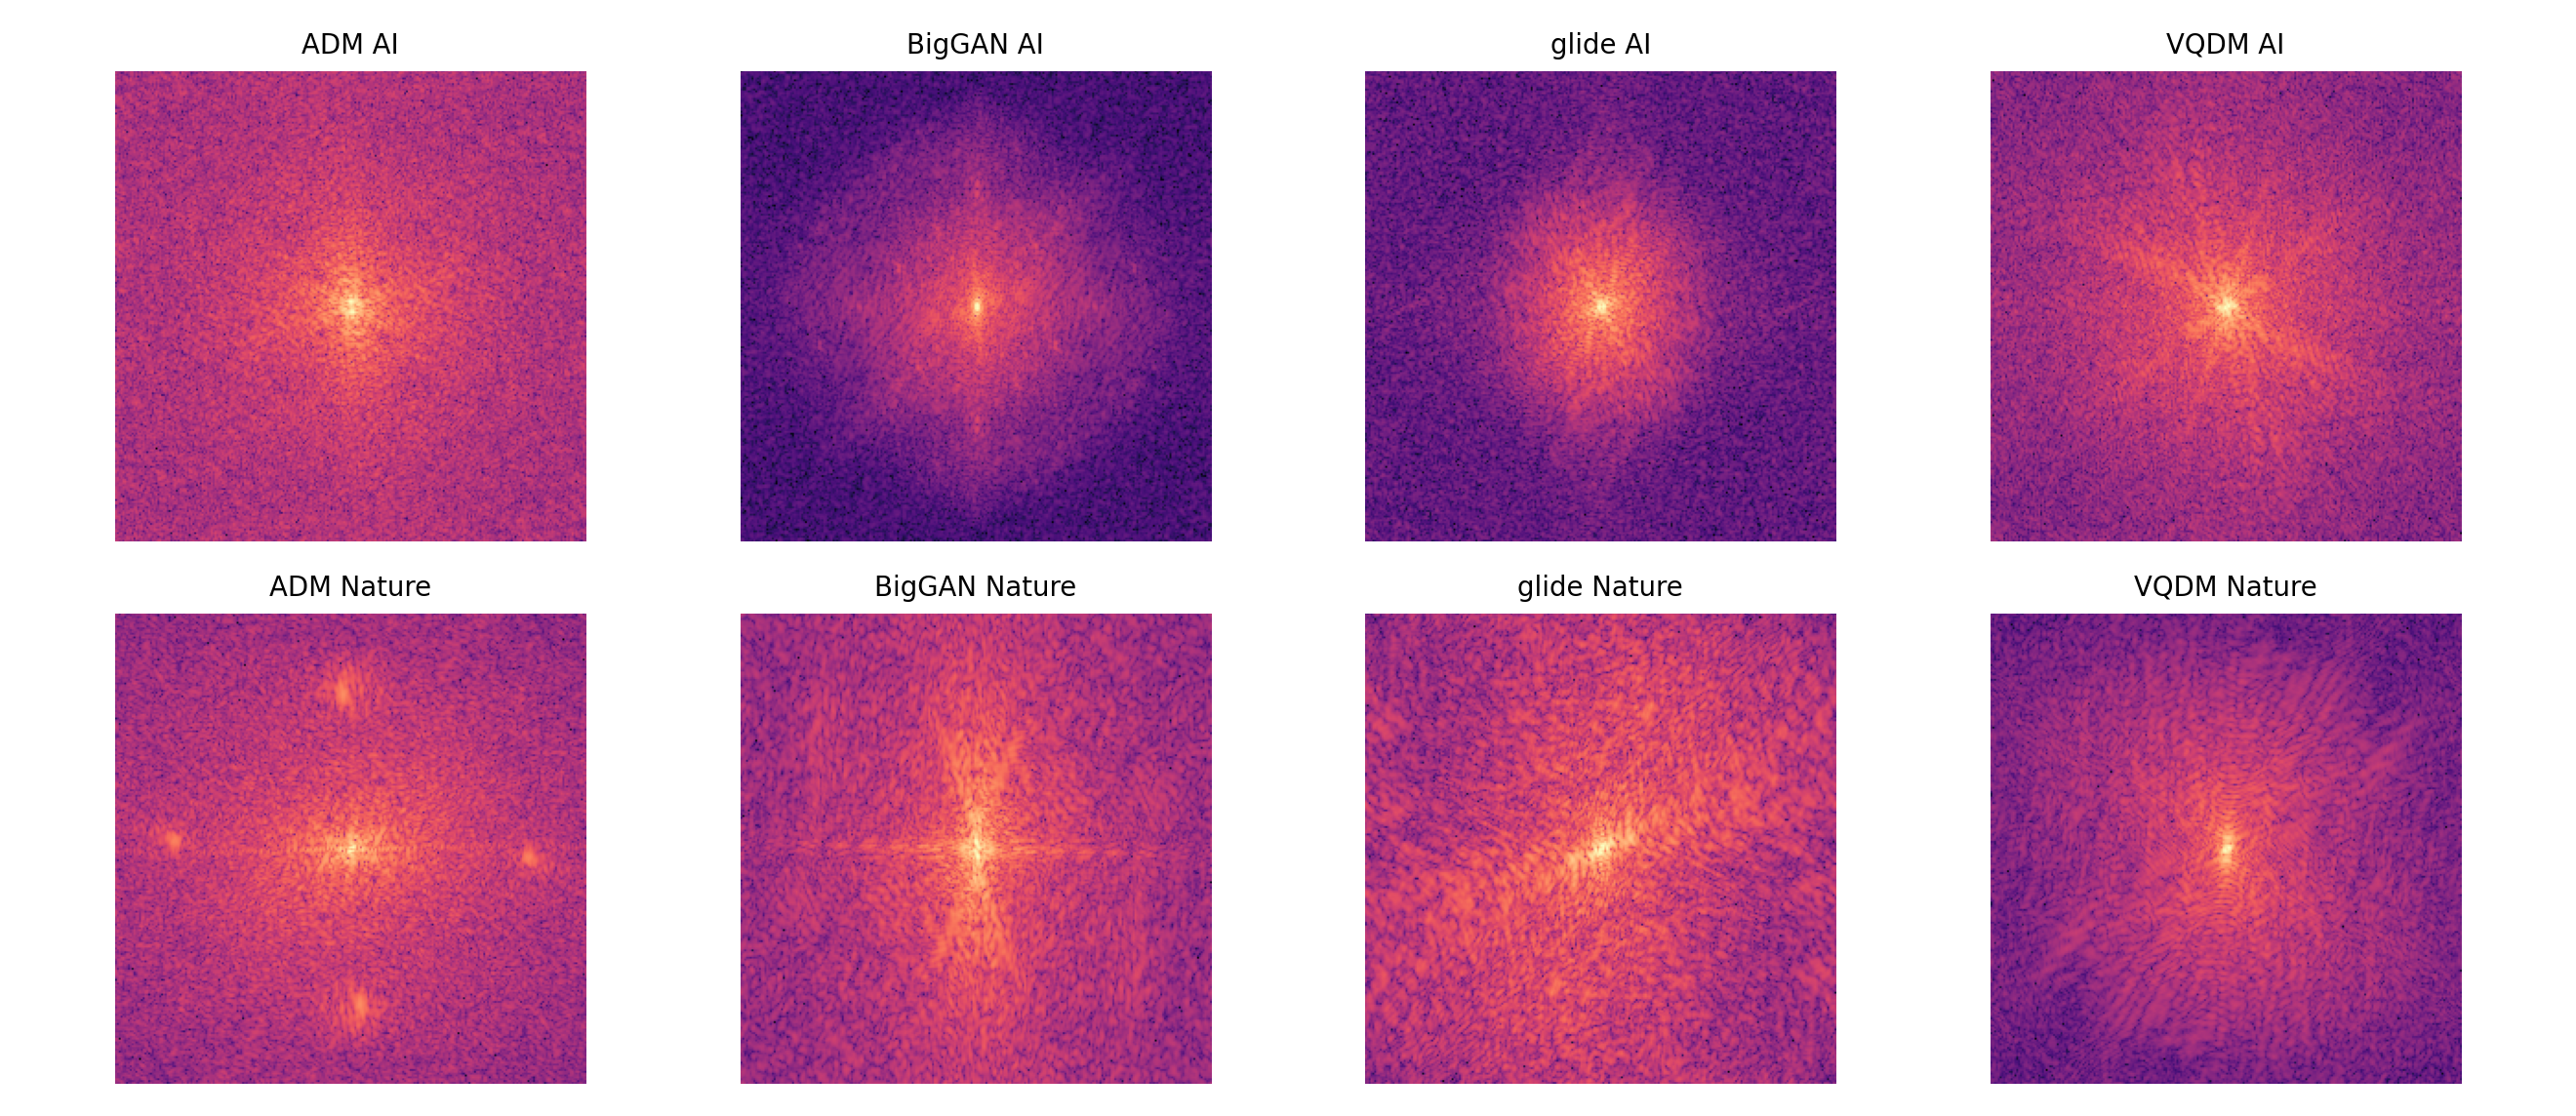
\includegraphics[width=\linewidth]{figures/spectrum_examples.png}}{\fbox{missing}}
  \caption{真实图像与不同生成源图像的频谱示例。该图用于说明频域指纹来自功率谱分布、频带能量和高频残差差异，而不是来自图像语义内容。}
  \label{fig:spectrum-examples}
\end{figure}

图~\ref{fig:all-model-comparison} 给出更完整的实验结果总览。与单一频域 profile 相比，融合频域 profile 不仅提高了二分类，也显著提高了生成源归因；与早期灰度 baseline 相比，第二轮 \texttt{fusion\_freq} 路线的提升不是来自单个模型偶然波动，而是在多个抽样比例和多个任务上同时出现。该图也展示了鲁棒训练分支的定位：\texttt{mild\_aug} 和 \texttt{robust\_aug} 可作为鲁棒性探索，但 clean F1 不超过 full fusion 主模型。因此，最终报告采用 \texttt{outputs\_v2\_full\_best} 作为主结果，并将训练增强、stable profile 和 leave-one-generator-out 作为严谨性补充。

\begin{figure}[H]
  \centering
  \IfFileExists{figures/model_comparison_macro_f1.png}{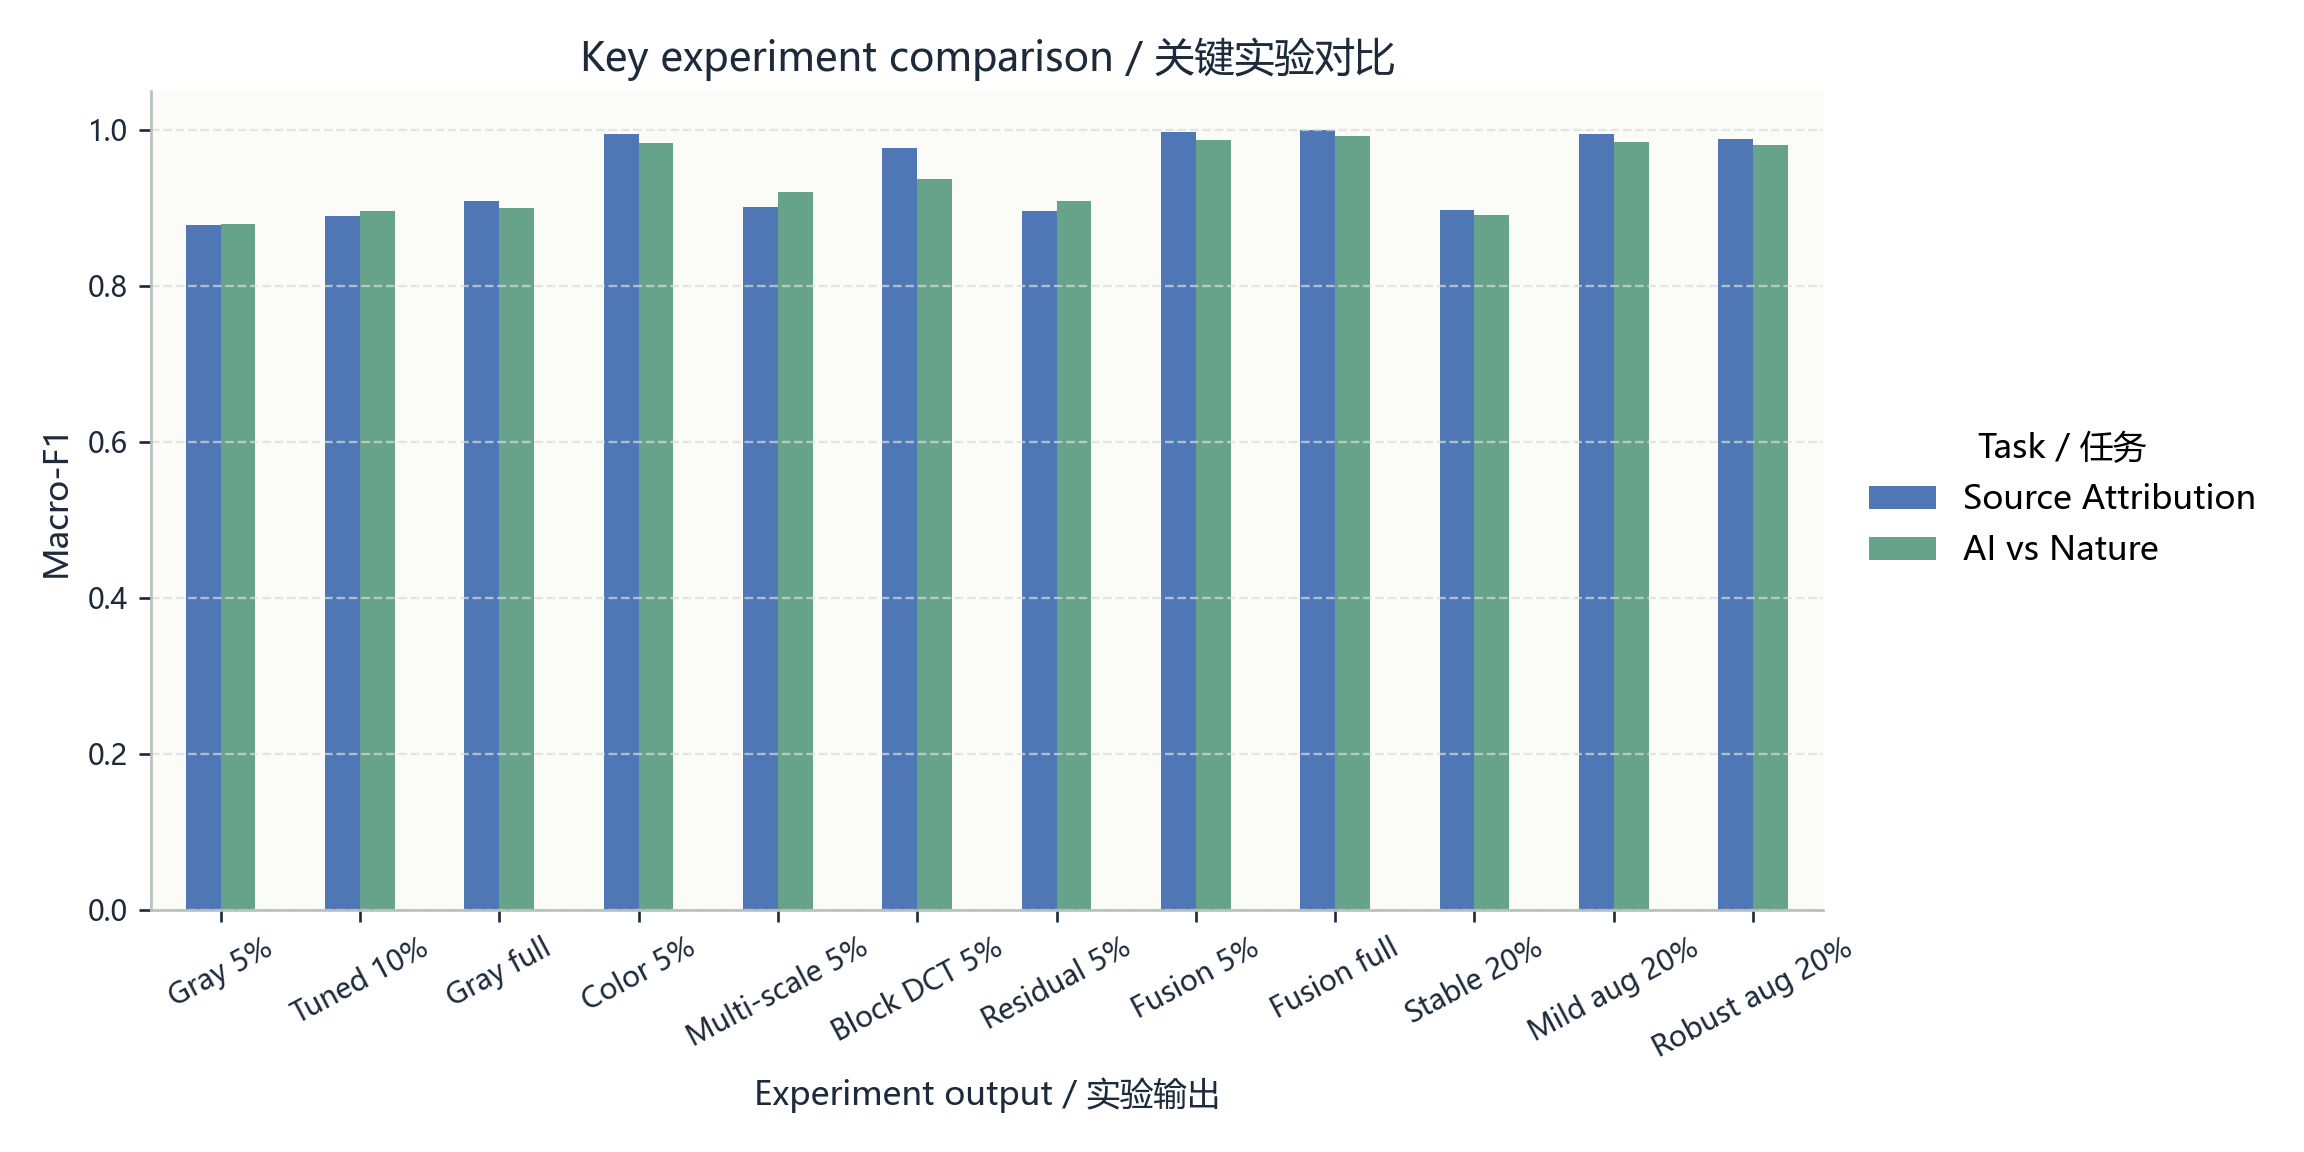
\includegraphics[width=\linewidth]{figures/model_comparison_macro_f1.png}}{\fbox{missing}}
  \caption{单一频域、融合频域、不同抽样比例和增强训练分支的整体 macro-F1 对比。该图用于补充说明最终主模型选择来自系统实验，而不是只根据单次运行决定。}
  \label{fig:all-model-comparison}
\end{figure}

\begin{table}[H]
  \centering
  \caption{单一频域 profile 与融合频域 profile 的代表性结果。}
  \label{tab:single-fusion}
  \begin{tabular}{lrrr}
    \toprule
    Profile & Binary F1 & Attr. F1 & Avg. F1 \\
    \midrule
    color\_freq 5\% & 0.9833 & 0.9942 & 0.9887 \\
    block\_dct 5\% & 0.9362 & 0.9766 & 0.9564 \\
    multiscale 5\% & 0.9204 & 0.9007 & 0.9105 \\
    residual 5\% & 0.9088 & 0.8951 & 0.9019 \\
    fusion 5\% & 0.9871 & 0.9967 & 0.9919 \\
    fusion full & \textbf{0.9913} & \textbf{0.9991} & \textbf{0.9952} \\
    \bottomrule
  \end{tabular}
\end{table}

表~\ref{tab:single-fusion} 进一步给出关键数值。可以看到，颜色频谱是最强的单一频域 profile，但仍低于同样 5\% 抽样下的融合频域。多尺度、块 DCT 和残差频谱单独使用时不一定最强，但它们提供了与颜色频谱不同的统计视角，因此在融合后能提高整体稳定性。图~\ref{fig:profile-selection} 则展示了参数和特征 profile 的筛选过程：\texttt{wide} LightGBM 在增强频谱配置中表现最好，也解释了为什么最终主路线固定为 \texttt{fusion\_freq + wide}。

\begin{figure}[H]
  \centering
  \IfFileExists{figures/enhanced_feature_search_macro_f1.png}{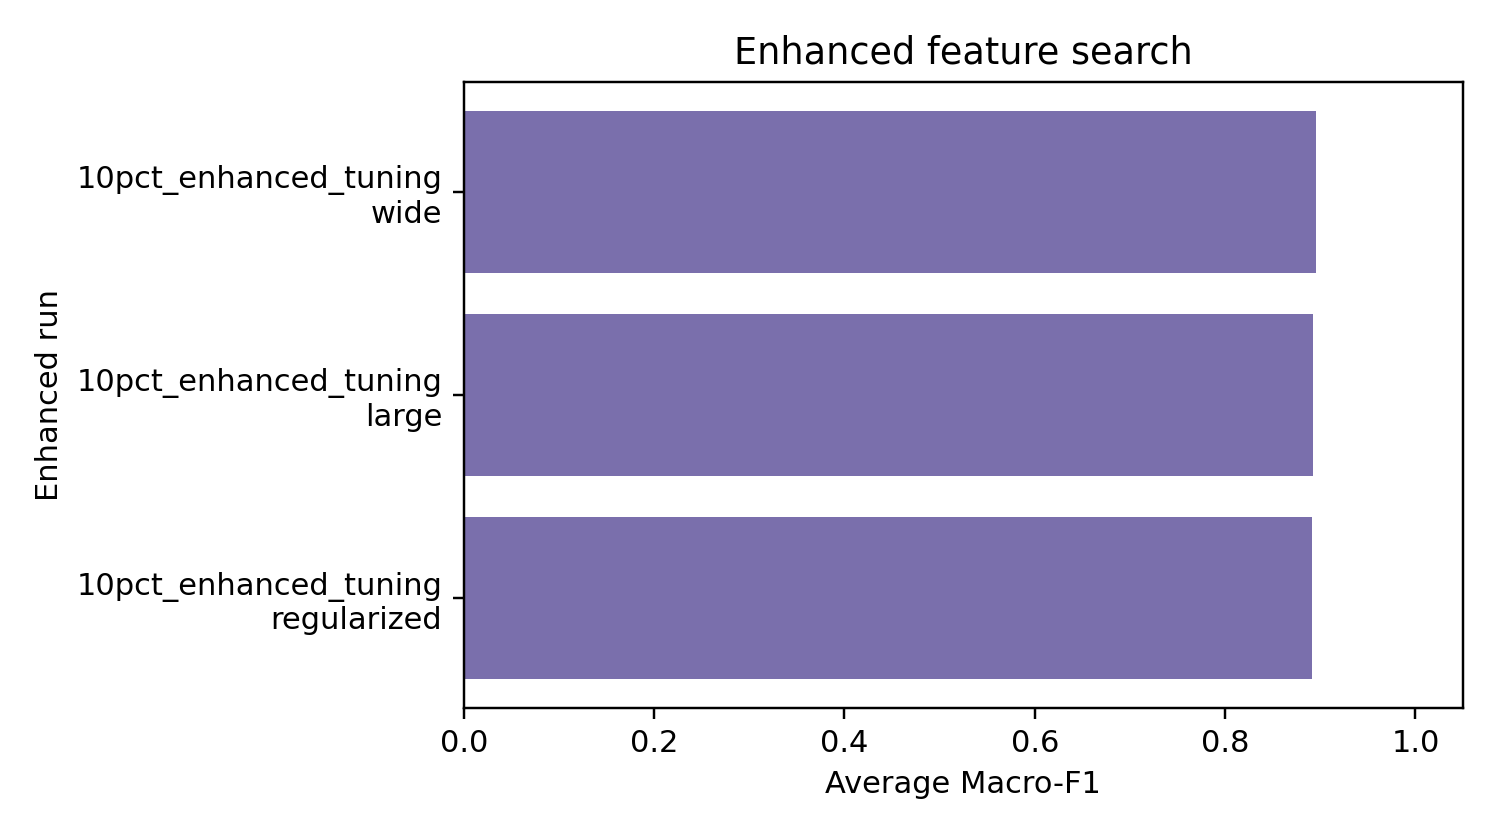
\includegraphics[width=0.49\linewidth]{figures/enhanced_feature_search_macro_f1.png}}{\fbox{missing}}
  \IfFileExists{figures/lgbm_tuning_binary_ai_vs_nature.png}{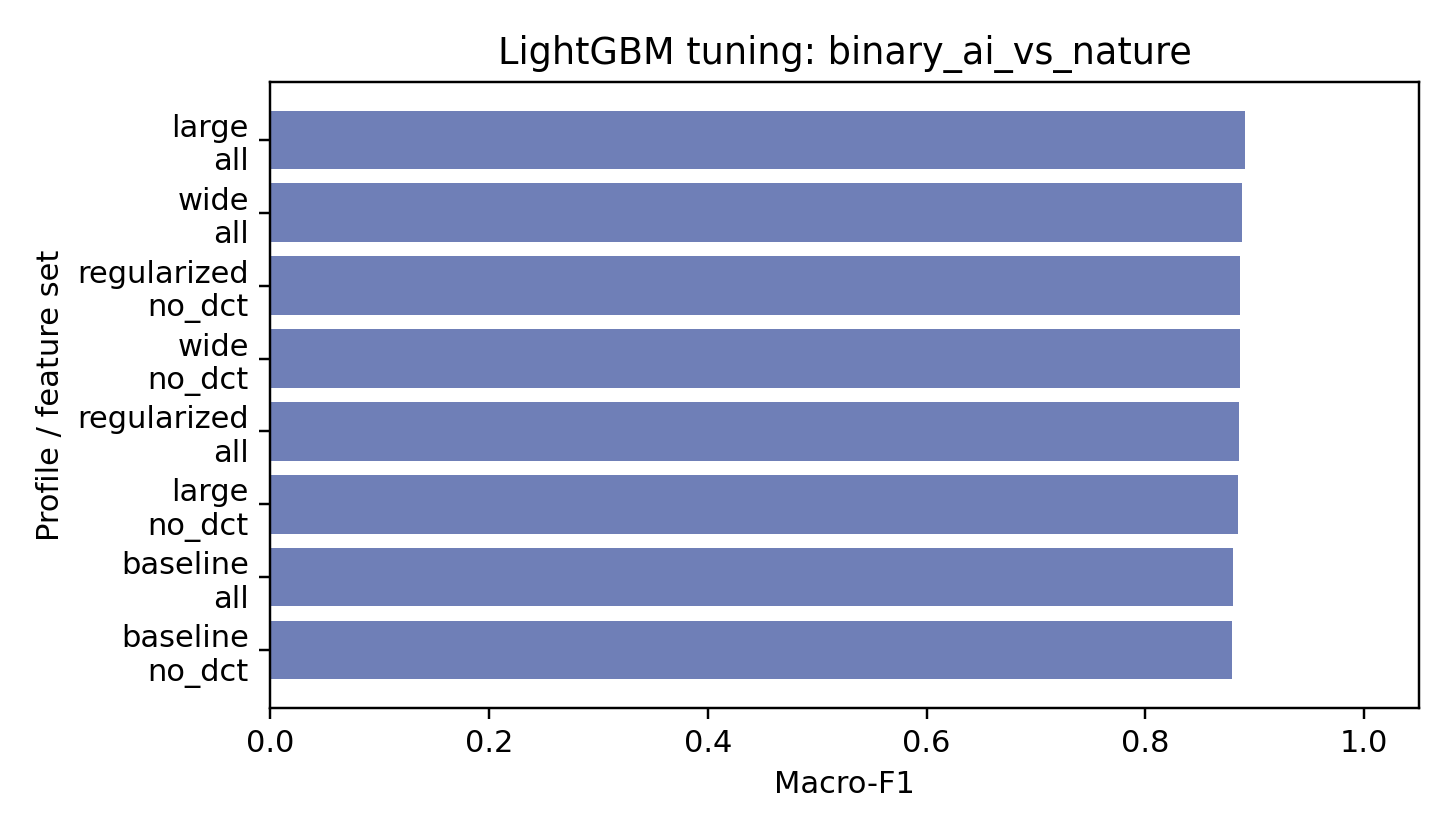
\includegraphics[width=0.49\linewidth]{figures/lgbm_tuning_binary_ai_vs_nature.png}}{\fbox{missing}}
  \caption{特征 profile 搜索与 LightGBM 参数调优结果。左图展示增强频域特征在不同 LightGBM profile 下的表现，右图展示二分类任务中的 LightGBM 调参对比。}
  \label{fig:profile-selection}
\end{figure}

\subsection{Feature Importance and Errors}
最终 full 模型在 48000 张二分类 validation 图像中误判 420 张，在 24000 张归因 validation 图像中误判 22 张。二分类错误更多来自 ADM 与 VQDM 的 AI 图像被判为 nature；归因错误主要集中在 ADM 与 VQDM 之间。这说明模型的主要难点不是 BigGAN 或 GLIDE，而是频谱统计更相近的生成源对。

\begin{figure}[H]
  \centering
  \IfFileExists{figures/confusion_ai_subsource_attribution_lightgbm.png}{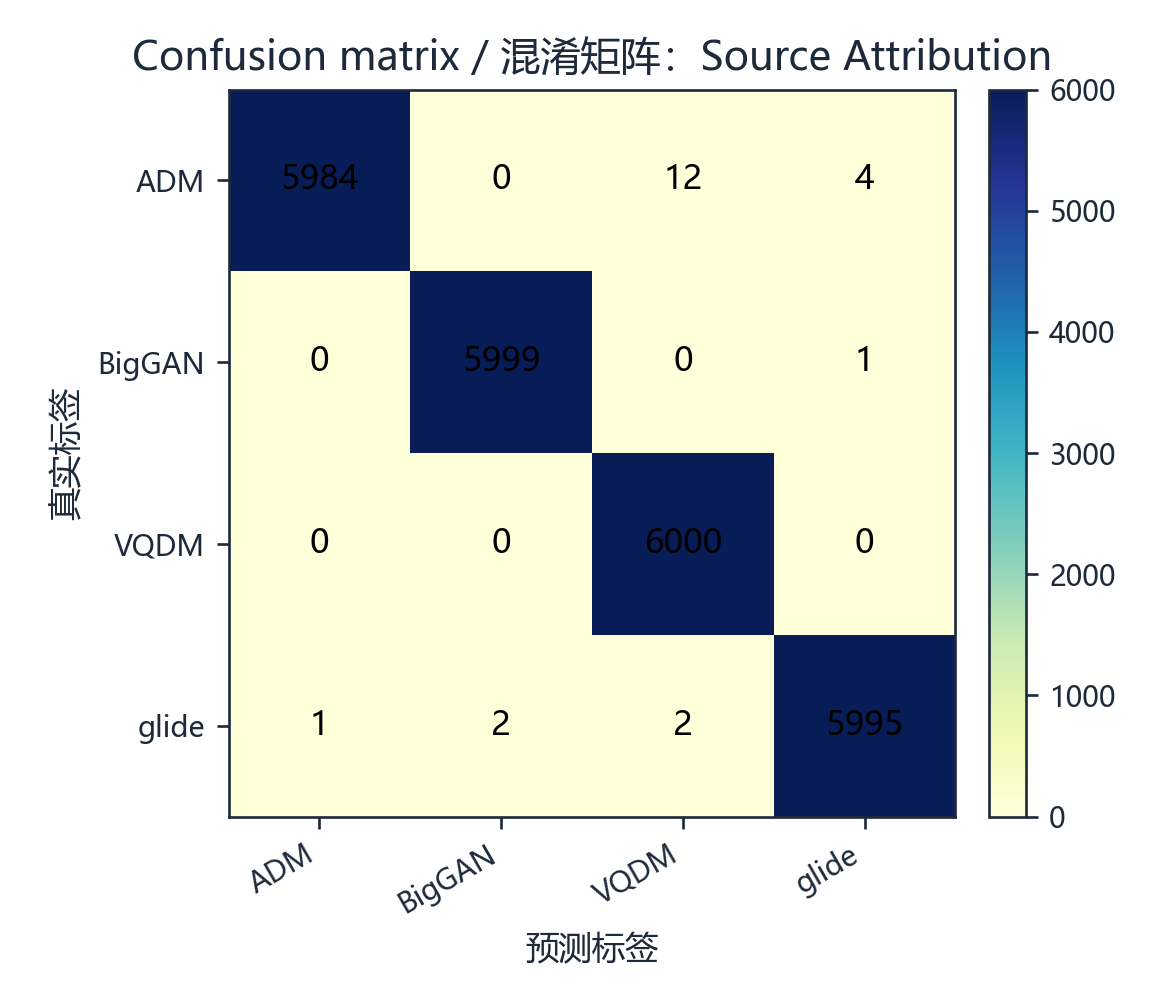
\includegraphics[width=\linewidth]{figures/confusion_ai_subsource_attribution_lightgbm.png}}{\fbox{missing}}
  \caption{最终 full 模型在生成源归因任务上的混淆矩阵。}
  \label{fig:confusion-attribution}
\end{figure}

\begin{figure}[H]
  \centering
  \IfFileExists{figures/feature_importance_binary_ai_vs_nature_top20.png}{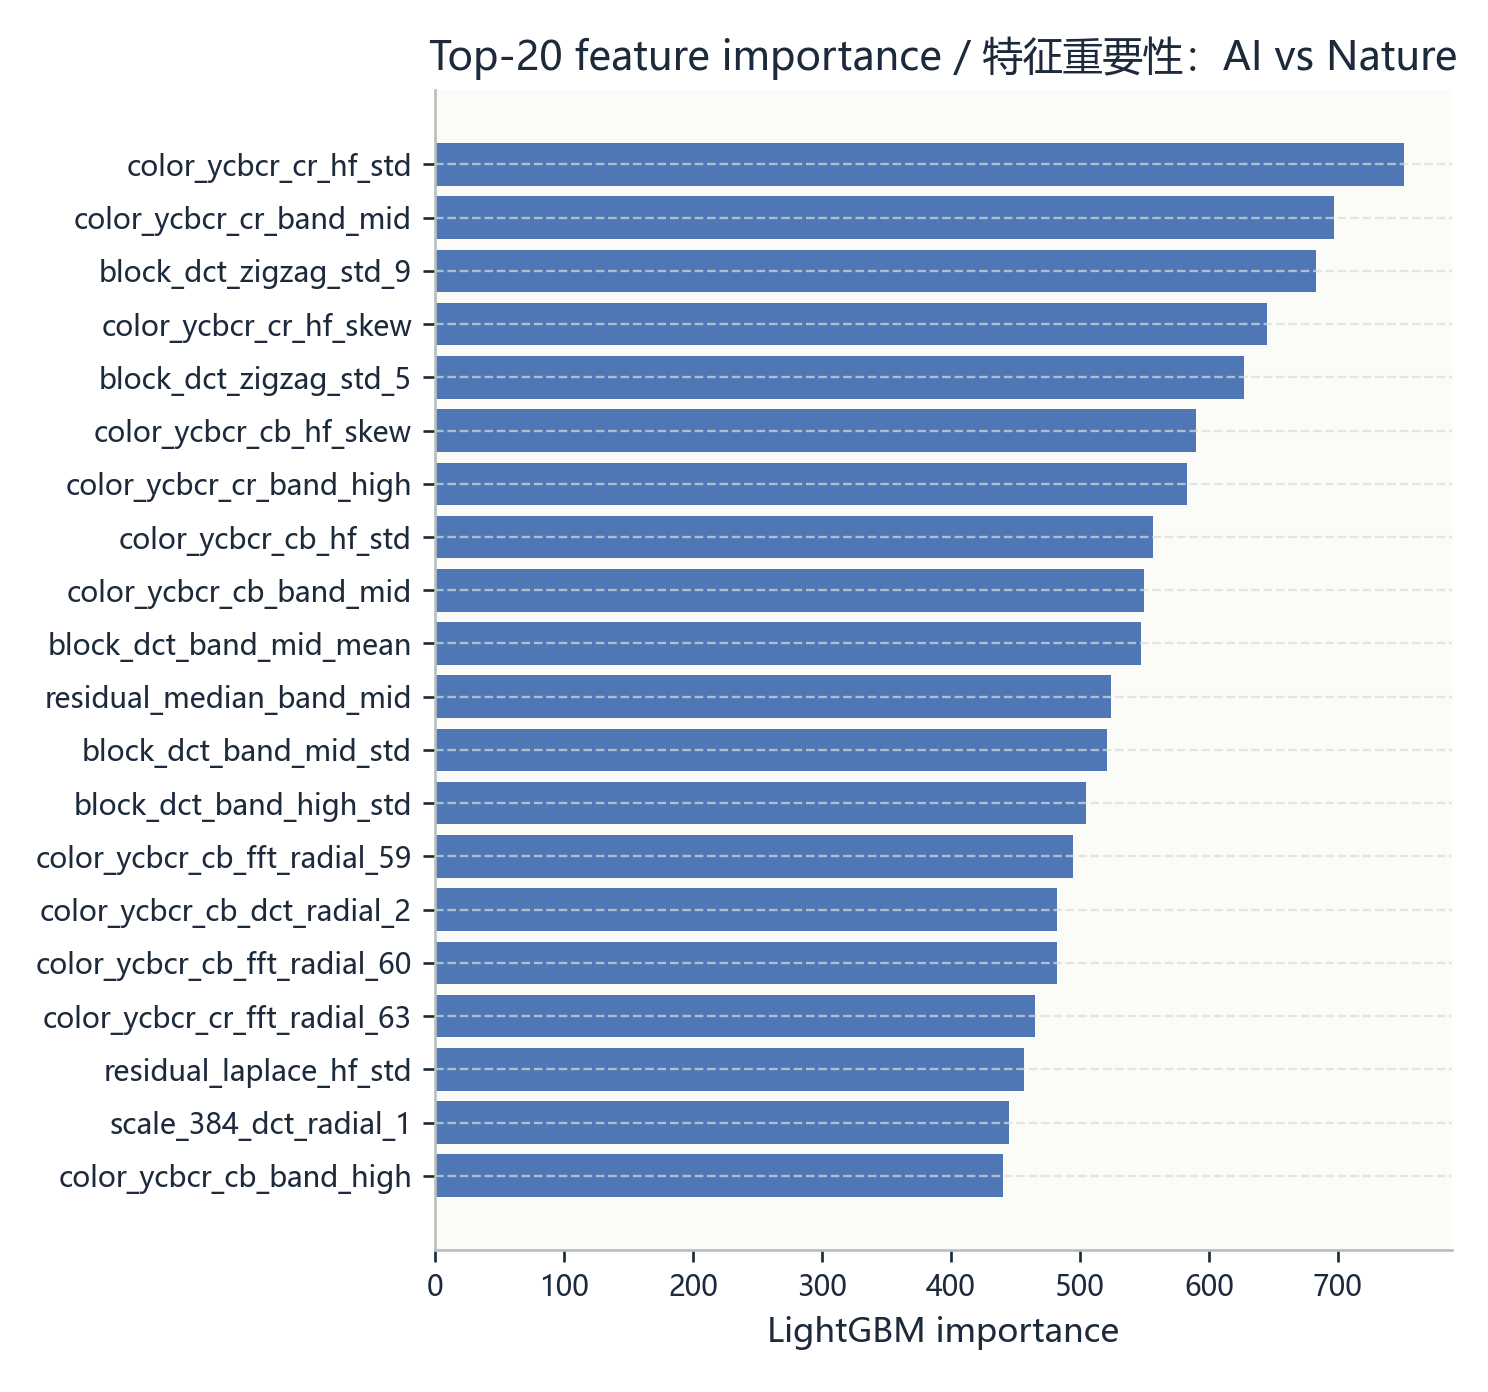
\includegraphics[width=\linewidth]{figures/feature_importance_binary_ai_vs_nature_top20.png}}{\fbox{missing}}
  \caption{二分类任务中的 Top-20 频域特征重要性。}
  \label{fig:feature-importance}
\end{figure}

特征重要性进一步支持了“颜色频谱 + 局部 DCT + 残差统计”共同起作用的结论。Top feature 中既包含 YCbCr 通道的高频标准差、band energy 和径向 DCT 统计，也包含 block-DCT 中高频 AC 能量和 residual median 高频统计。这说明模型并不是只依赖单个阈值或单个频段，而是在多个互补频域视角上形成判别边界。对于二分类，颜色通道高频和中高频能量最有用，符合生成图像在颜色噪声、去噪残差和上采样纹理上存在系统偏差的假设。对于归因任务，特征重要性更偏向生成器特定的频谱形态，例如 ADM/VQDM 的残差频谱差异、BigGAN 的局部纹理周期性和 GLIDE 的频带能量分布。

错误分析也说明模型的失败不是随机噪声。二分类中的误判主要出现在 ADM 与 VQDM：部分 AI 图像被判成 nature，说明这些生成源在某些样本上的频谱更接近自然图像统计；少量 nature 被判成 AI，通常具有强纹理、重复边缘或压缩伪影，这些模式会被浅层频谱模型误认为生成痕迹。归因任务中，BigGAN 和 GLIDE 几乎不混淆，说明它们的频谱签名较稳定；ADM 与 VQDM 的混淆更多，说明这两个扩散/量化扩散相关生成源在全局功率谱和残差噪声上更相近。因此，后续提升归因任务的关键不是继续扩大已有样本，而是设计专门区分 ADM/VQDM 的专家特征或 pairwise classifier。

从可解释性角度看，错误样本列表比单一准确率更重要。项目导出的 \texttt{prediction\_errors.csv} 记录了路径、真实标签、预测标签和模型置信度，可用于检查高置信度错误是否集中在特定生成器或特定图像类型。如果高置信度错误集中在纹理复杂的 nature 图像，说明模型把自然纹理误认为生成伪影；如果集中在某个 AI 生成源，说明该生成源的频谱分布与训练中其它源不一致。这样的分析能把“模型错了多少”进一步转化为“模型为什么错”，也使报告中的可解释性不只停留在 feature importance 条形图。

\subsection{Robustness and Generalization}
鲁棒性实验直接加载 \texttt{outputs\_v2\_full\_best} 的最佳模型，不重新训练。表~\ref{tab:robustness} 显示：\texttt{fusion\_freq} 在 clean 子集上接近满分，但 JPEG、resize 和 Gaussian noise 会显著改变高频与颜色频谱统计，从而造成预测分布偏移。旧灰度 baseline 的 clean 分数较低，但在部分 JPEG/noise 场景更稳，说明 clean 性能和 degraded 稳定性之间存在取舍。

\begin{table}[H]
  \centering
  \caption{20\% validation 上的鲁棒性诊断 macro-F1。}
  \label{tab:robustness}
  \begin{tabular}{lrr}
    \toprule
    Setting & Binary & Attribution \\
    \midrule
    clean & 0.9908 & 0.9992 \\
    JPEG 95 & 0.6607 & 0.2952 \\
    JPEG 50 & 0.5666 & 0.2526 \\
    resize 0.5 & 0.3671 & 0.1551 \\
    resize 1.5 & 0.8136 & 0.6282 \\
    noise 2 & 0.7481 & 0.1887 \\
    noise 10 & 0.3377 & 0.1000 \\
    \bottomrule
  \end{tabular}
\end{table}

\begin{figure}[H]
  \centering
  \IfFileExists{figures/robustness_comparison_binary_ai_vs_nature.png}{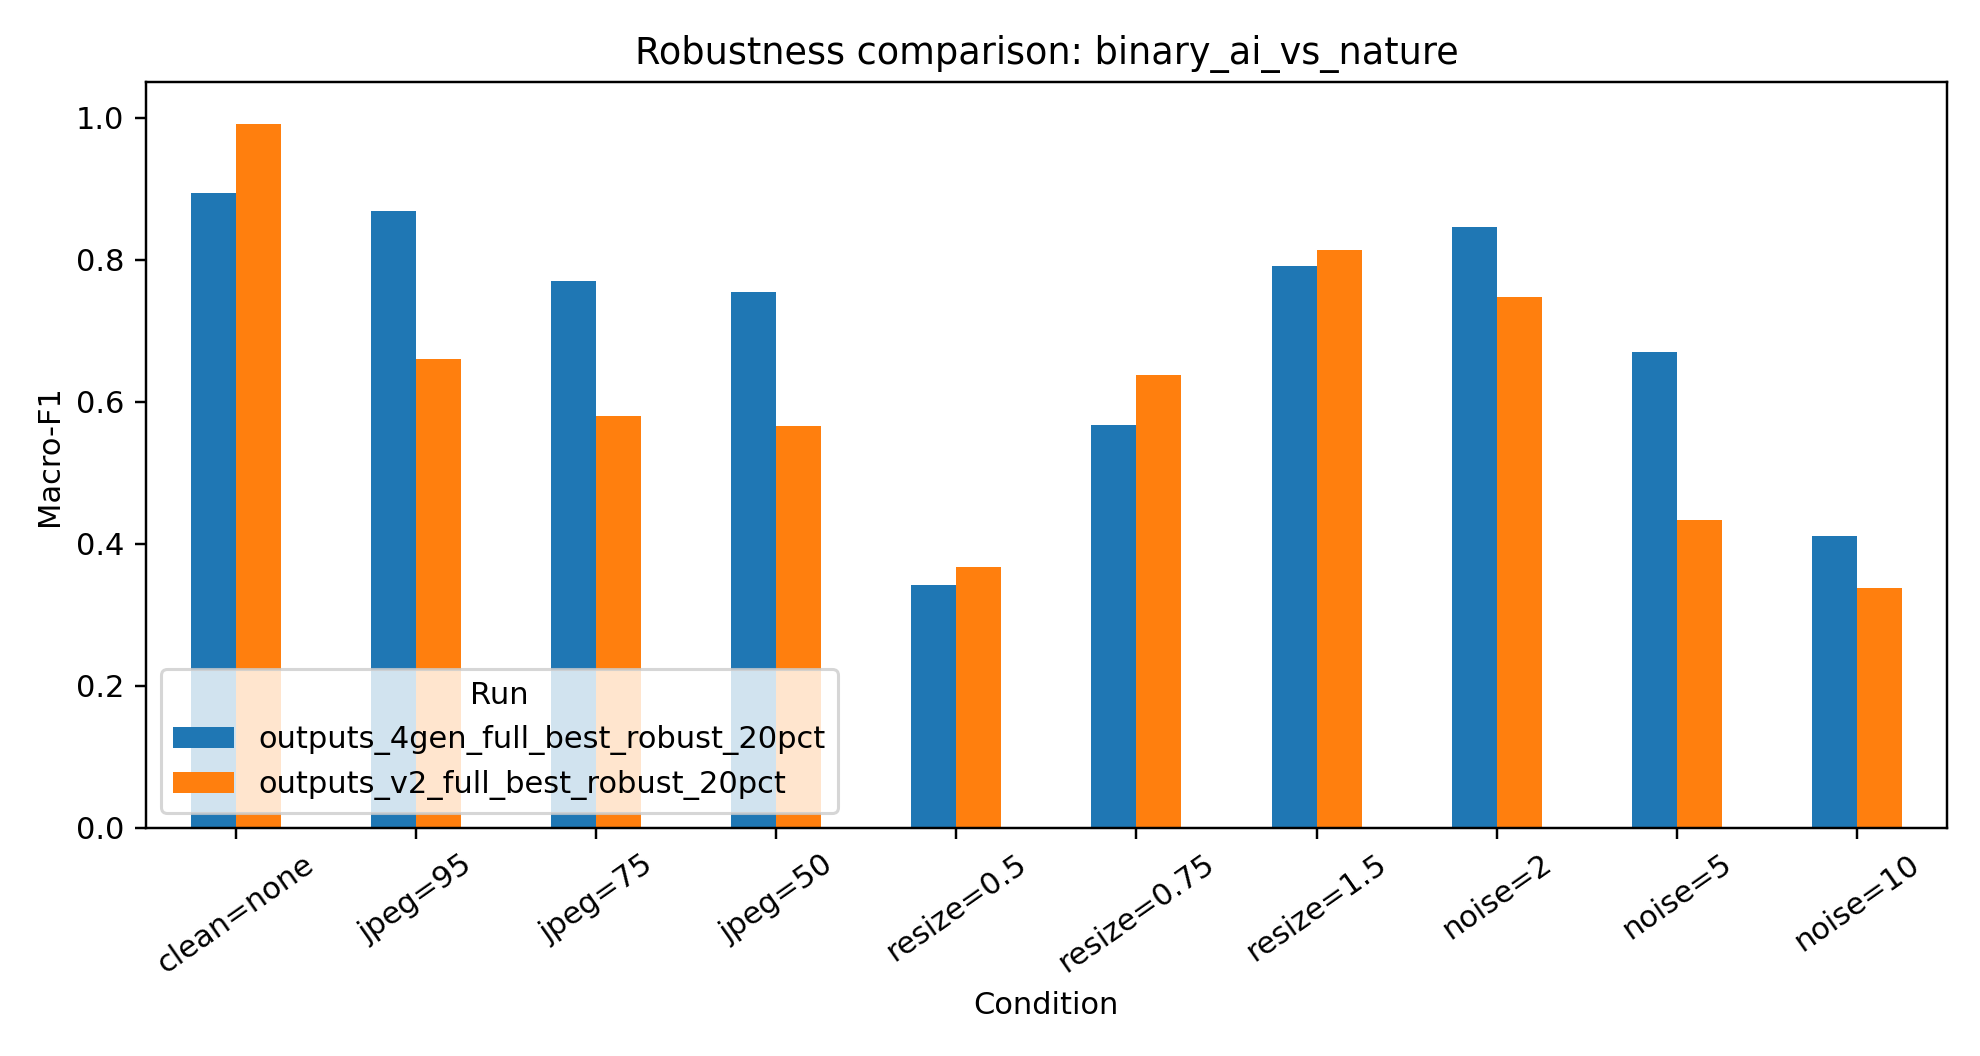
\includegraphics[width=0.49\linewidth]{figures/robustness_comparison_binary_ai_vs_nature.png}}{\fbox{missing}}
  \IfFileExists{figures/robustness_comparison_ai_subsource_attribution.png}{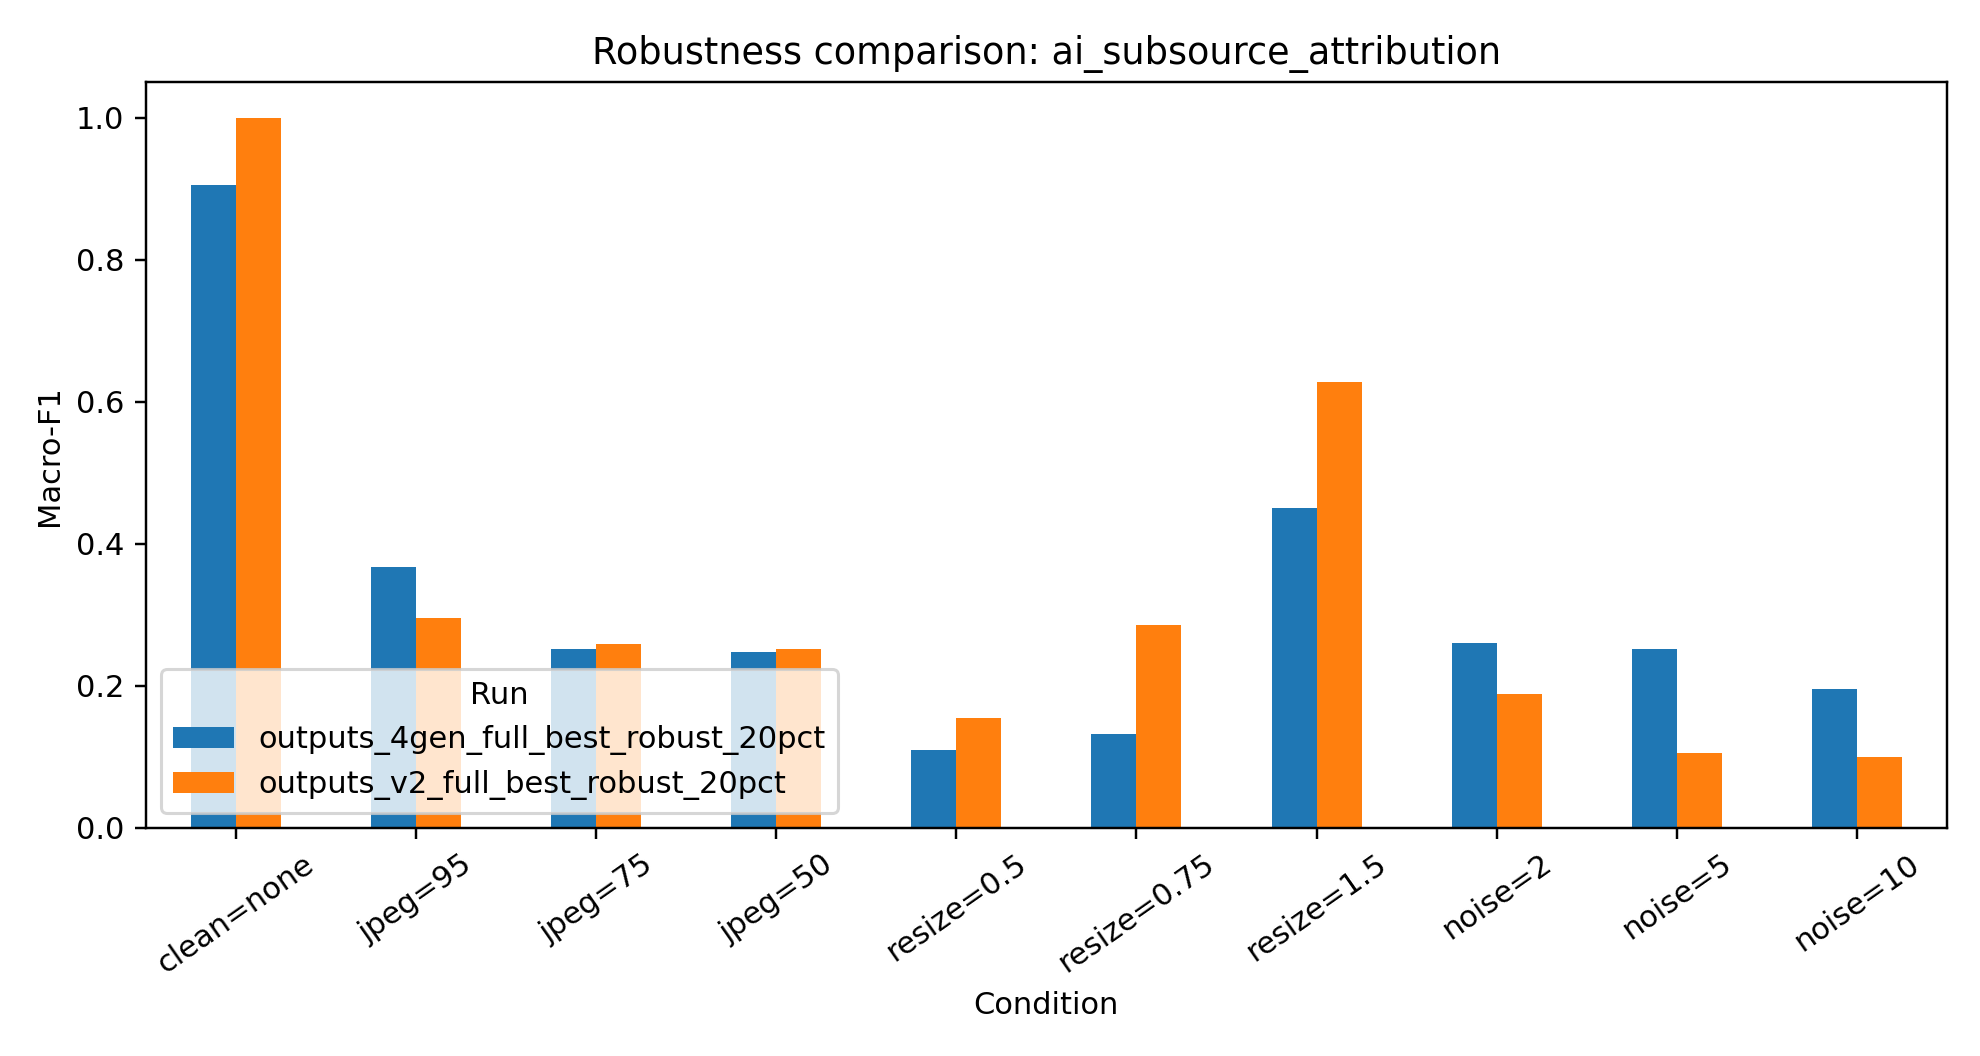
\includegraphics[width=0.49\linewidth]{figures/robustness_comparison_ai_subsource_attribution.png}}{\fbox{missing}}
  \caption{当前 \texttt{fusion\_freq} 最佳模型与旧灰度 baseline 的 degraded validation 对照。}
  \label{fig:robustness-comparison}
\end{figure}

鲁棒性结果说明，clean performance 不能直接等价为真实部署场景中的稳定性。JPEG 压缩会量化局部 DCT 系数并抑制高频细节，恰好破坏 \texttt{fusion\_freq} 中贡献较大的颜色高频和 block-DCT 统计；因此 JPEG 95 已经使二分类 F1 从 0.9908 降到 0.6607，JPEG 50 下进一步下降。缩放扰动的影响具有方向性：resize 0.5 会丢失细节并重采样高频，二分类 F1 降到 0.3671；resize 1.5 虽然也改变频谱，但保留了更多原始结构，因此二分类 F1 仍有 0.8136。高斯噪声则直接向高频区域注入随机能量，使模型学习到的“生成残差”与外加噪声混合，导致强噪声下性能明显下降。

归因任务在 degraded 场景下退化更严重，这与任务定义有关。二分类只需要判断“是否 AI”，仍可能利用部分残留的通用频谱偏差；归因任务需要区分 ADM、BigGAN、VQDM 和 GLIDE 的细粒度签名，一旦 JPEG、resize 或 noise 抹平生成器间差异，类别边界就会快速变得不稳定。这个现象也是本文的重要负面结果：频域融合可以显著提升 clean 归因，但它对后处理更敏感。报告中因此不把鲁棒性实验写成“已解决”，而是作为失效模式诊断。

旧灰度 baseline 在 clean 分数上远低于 \texttt{fusion\_freq}，但在部分 degraded 条件下并没有同等幅度崩溃。这说明较简单的低维灰度频谱特征可能更少依赖颜色高频细节，因而在强压缩或噪声下有时更稳。后续如果目标从课程实验转向真实平台部署，合理路线不是继续单纯提高 clean F1，而是组合三类策略：训练时加入压缩、缩放和噪声增强；测试时对多个扰动版本做特征平均或投票；在特征层降低对极高频颜色统计的依赖，增加更稳健的低/中频和 DCT 结构统计。

进一步的 4-generator 扩展实验显示，\texttt{stable\_freq} 的二分类 clean F1 只有 0.8903，但 degraded 平均 F1 达到 0.6493；\texttt{fusion\_freq} full best 的二分类 clean F1 为 0.9908，但 degraded 平均 F1 为 0.5717。鲁棒训练分支 \texttt{robust\_aug} 在归因 degraded 平均 F1 上提升到 0.6347，但 clean F1 低于主模型，因此仅作为 tradeoff 分析。

\begin{figure}[H]
  \centering
  \IfFileExists{figures/robustness_tradeoff_binary_ai_vs_nature.png}{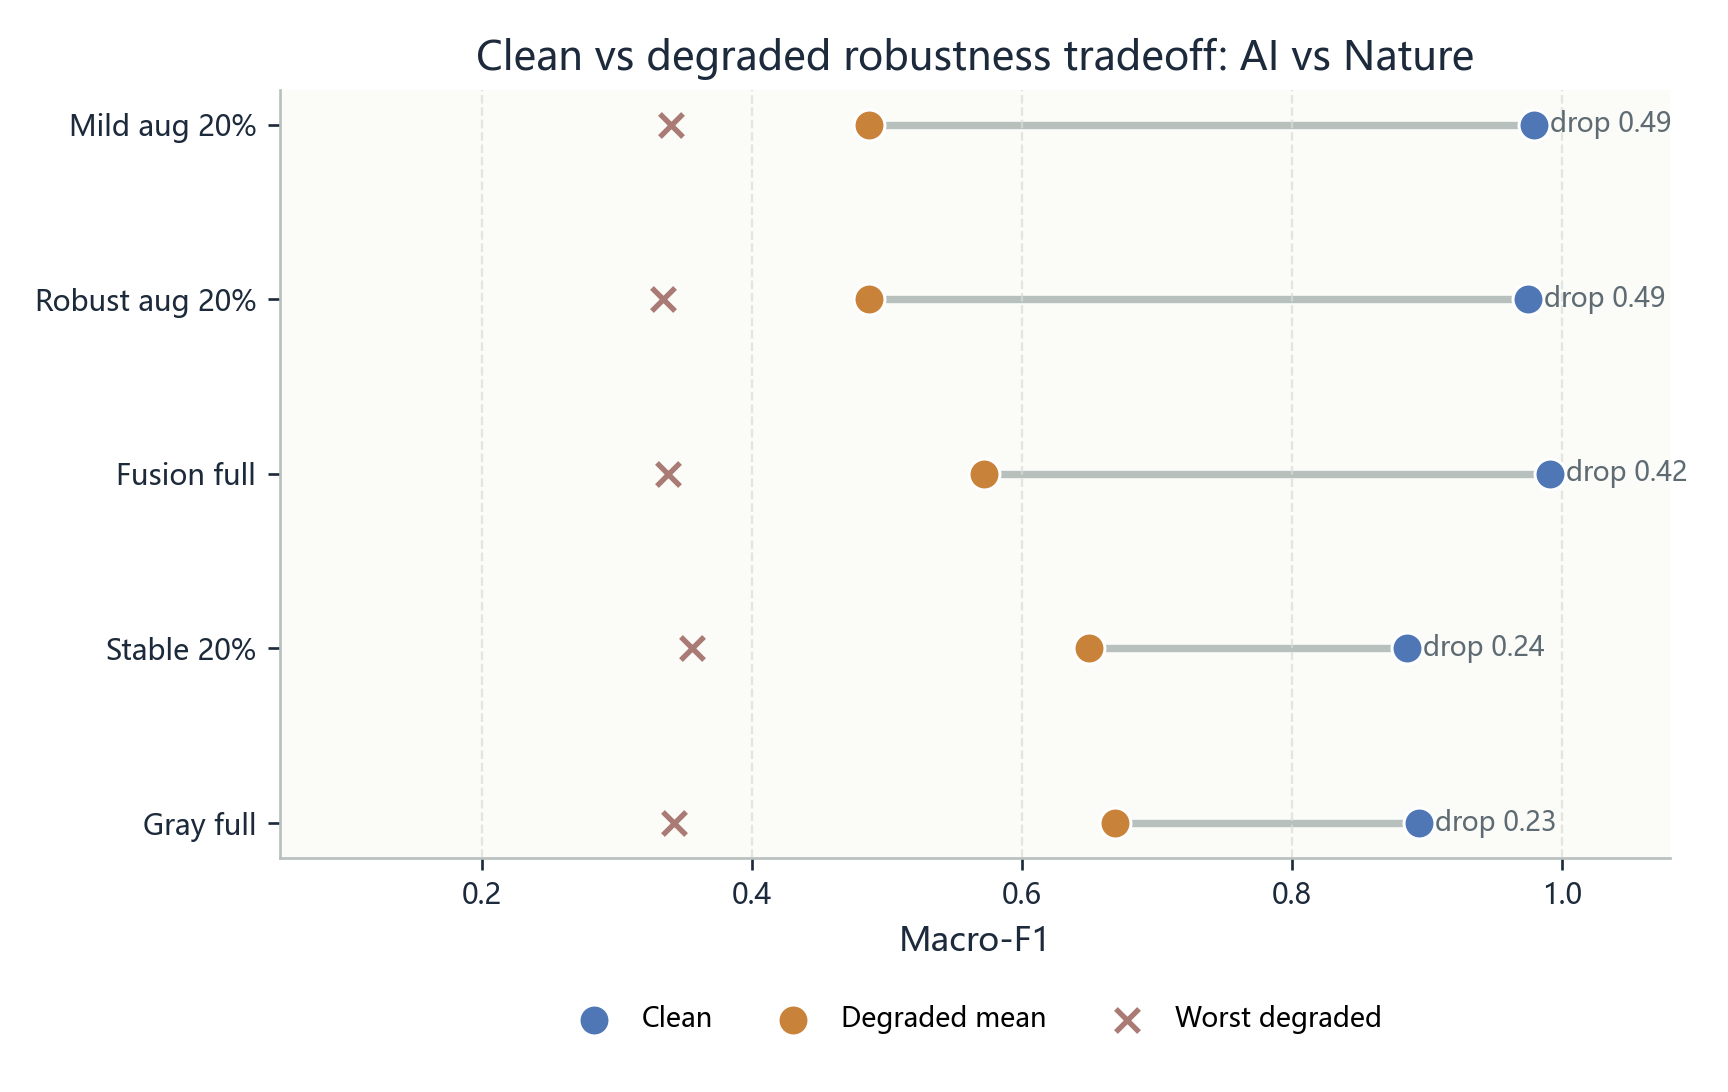
\includegraphics[width=0.49\linewidth]{figures/robustness_tradeoff_binary_ai_vs_nature.png}}{\fbox{missing}}
  \IfFileExists{figures/logo_generalization_macro_f1.png}{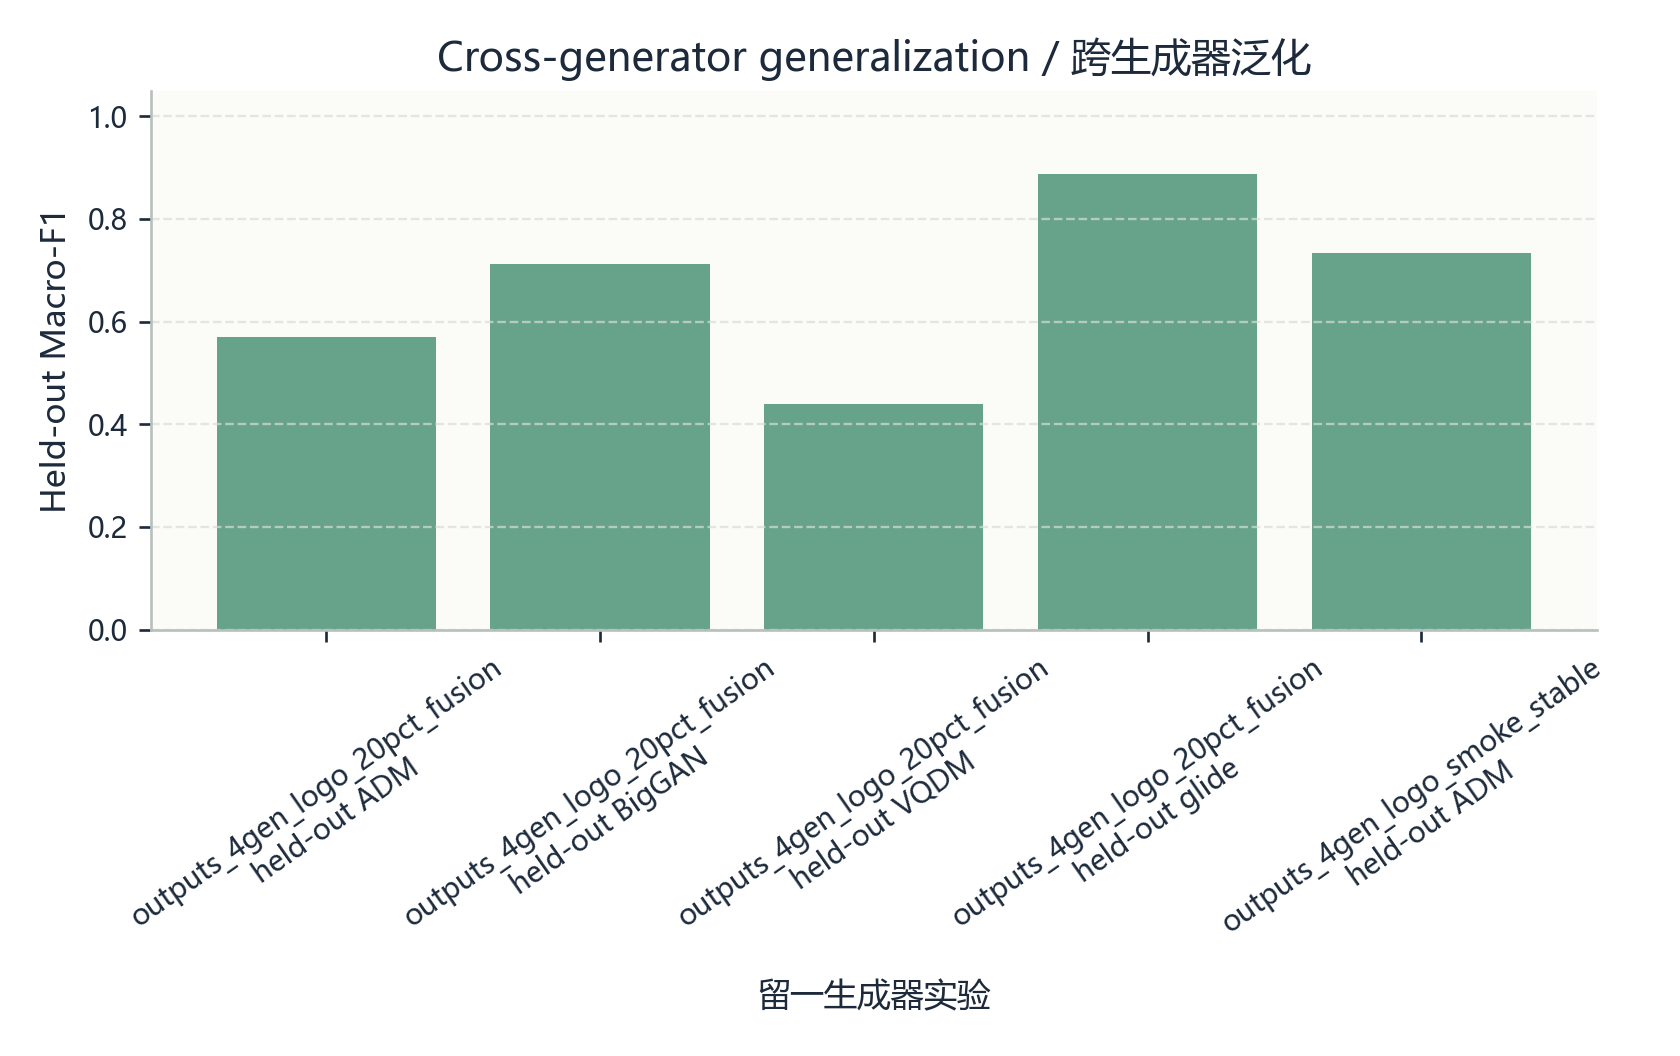
\includegraphics[width=0.49\linewidth]{figures/logo_generalization_macro_f1.png}}{\fbox{missing}}
  \caption{左：clean 与 degraded 平均 F1 的取舍；右：leave-one-generator-out 泛化结果。}
  \label{fig:tradeoff-logo}
\end{figure}

留一生成器泛化实验只用三个生成源训练二分类器，并在被留出的生成源上测试。结果显示 held-out GLIDE 的 macro-F1 为 0.8877，BigGAN 为 0.7120，ADM 为 0.5696，VQDM 仅为 0.4386。这说明模型确实学习到部分通用 AIGC 指纹，但也明显依赖已见生成器的特定频谱签名。

留一实验的排序也提供了对生成源差异的解释。GLIDE 被留出时仍能取得较高 F1，说明它与其余生成源共享的频谱偏差较多；VQDM 被留出时 F1 最低，说明它的频谱统计与训练中可见生成源差异较大，或更容易与真实图像统计接近。这个结果提醒我们，四生成源 clean 测试上的高分并不能自动推广到未见生成器。若要扩展为更严格的 benchmark，应补齐 Midjourney、Wukong、Stable Diffusion V1.4/V1.5 等生成源，并把“训练可见生成器、测试未见生成器”作为主要评价协议之一。

\subsection{Confidence and Rejection}
置信度分析导出预测概率、margin 与 entropy，并计算 coverage-accuracy 曲线。二分类任务中 BigGAN 的准确率最高，为 0.9953，ADM 与 VQDM 的平均置信度较低；归因任务中 ADM 的准确率最低，为 0.9973。这与错误分析一致：ADM/VQDM 是最主要的系统性混淆来源。拒识曲线表明，若允许模型在低置信度样本上输出“不确定”，高覆盖率下仍能保留较高准确率，因此 confidence 可以作为实际部署时的风险控制信号。

置信度分析的作用不是继续提高分数，而是为模型可信度提供可操作的解释。在实际应用中，检测器不一定必须对每张图片给出二元结论；当 margin 较小或 entropy 较高时，可以把样本交给人工复核或更强的深度模型。本文导出的 low-confidence list 和 high-confidence wrong list 可以帮助定位两类风险：前者代表模型本身不确定的边界样本，后者代表模型非常自信但判断错误的系统性盲区。对于课程项目，这部分补充了从“模型准确”到“模型何时不可靠”的分析链条。

\begin{figure}[H]
  \centering
  \IfFileExists{figures/confidence_coverage_binary_ai_vs_nature.png}{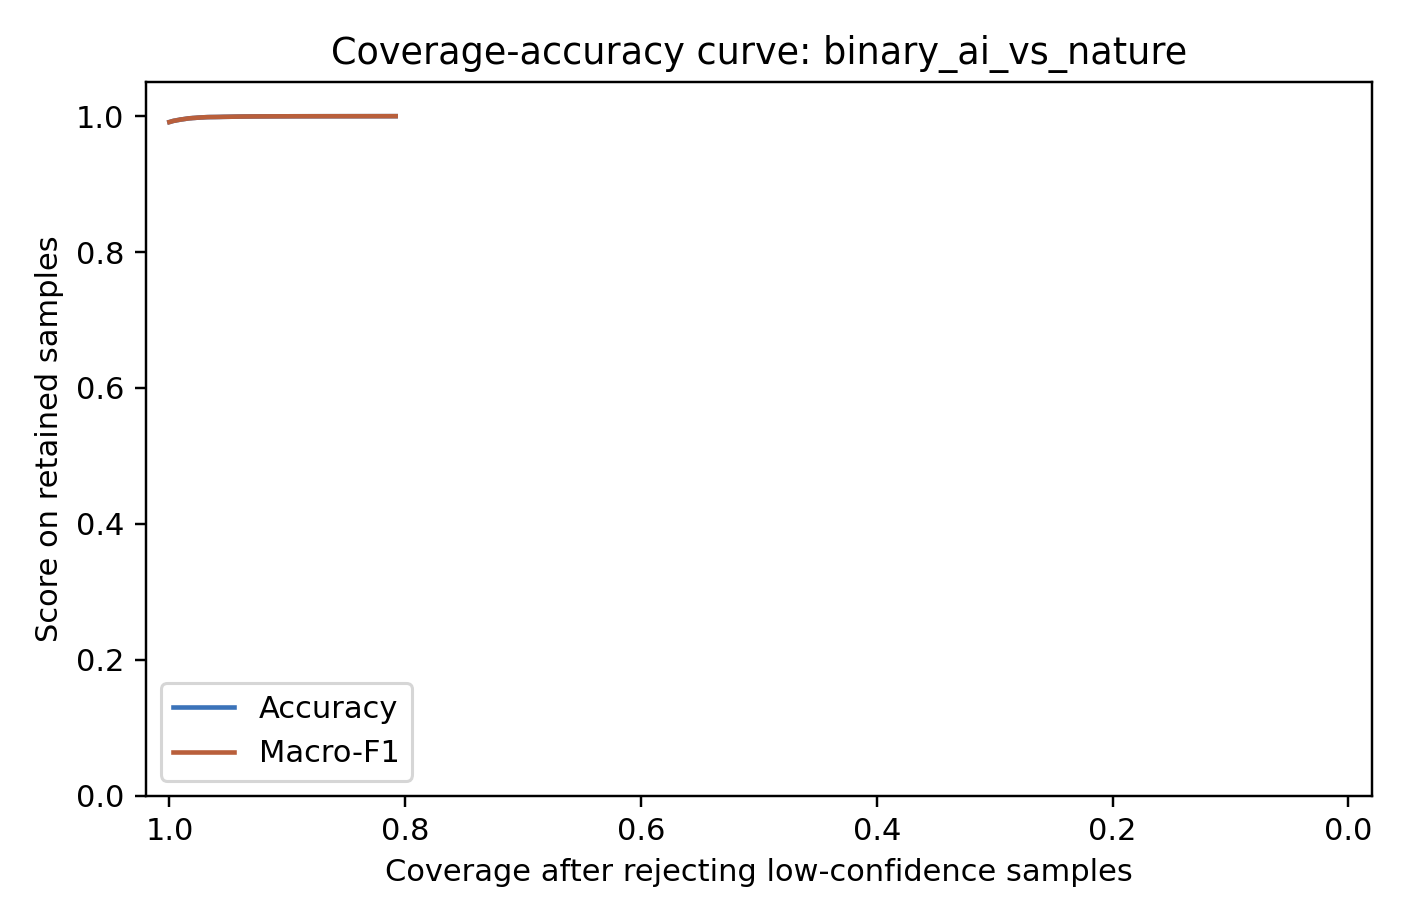
\includegraphics[width=0.49\linewidth]{figures/confidence_coverage_binary_ai_vs_nature.png}}{\fbox{missing}}
  \IfFileExists{figures/confidence_histogram_binary_ai_vs_nature.png}{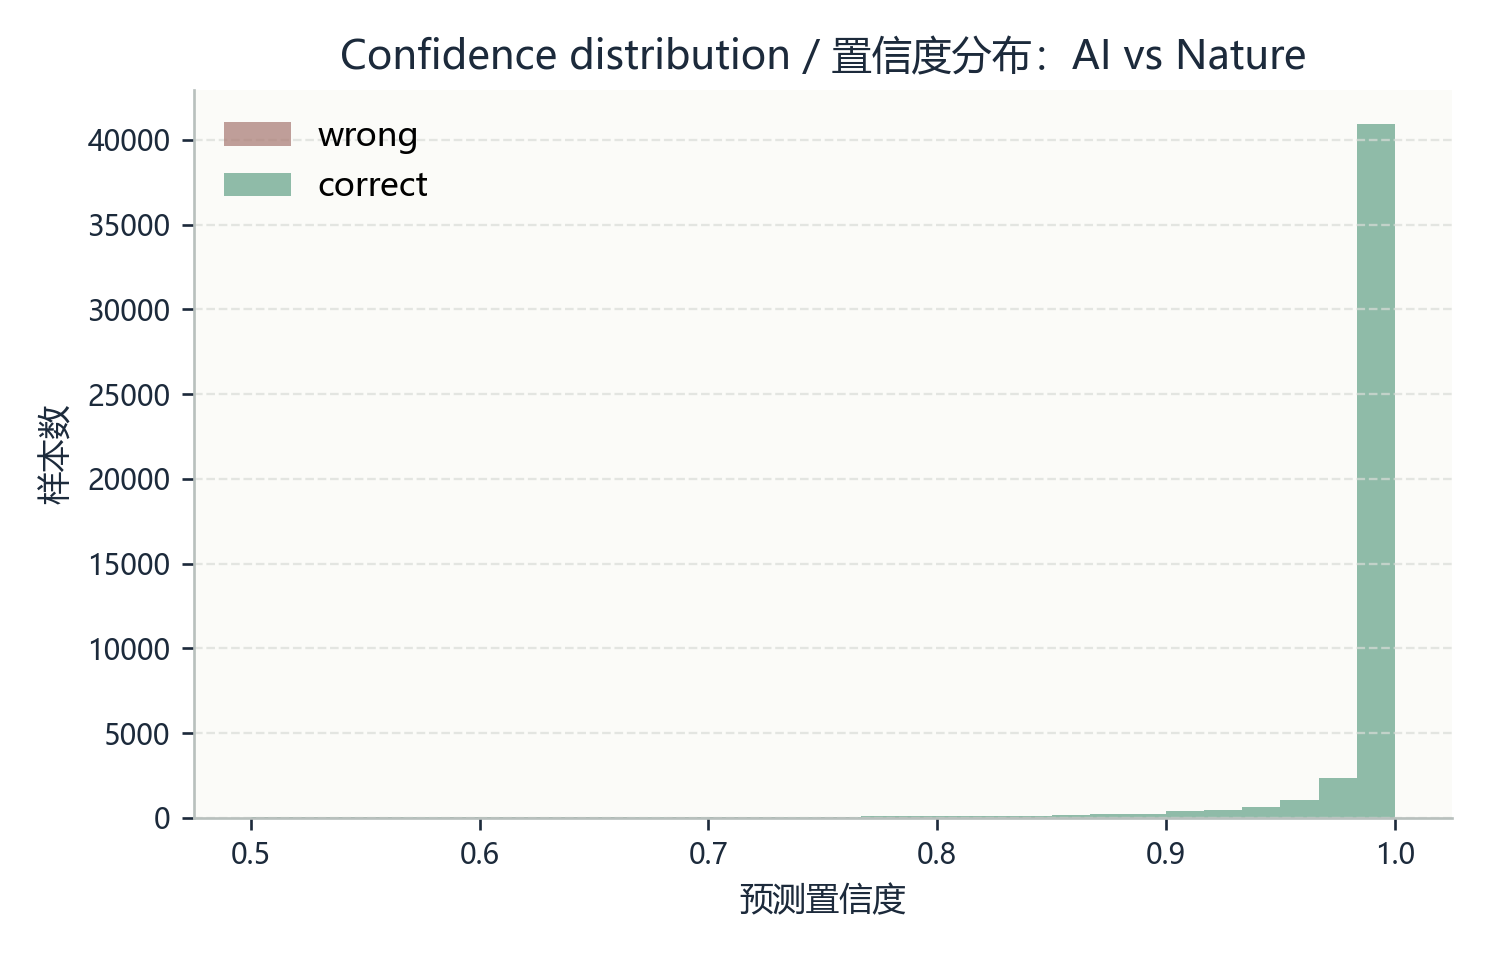
\includegraphics[width=0.49\linewidth]{figures/confidence_histogram_binary_ai_vs_nature.png}}{\fbox{missing}}
  \caption{二分类任务的 coverage-accuracy 曲线与置信度分布。}
  \label{fig:confidence}
\end{figure}

\vspace{-0.4em}
\section{Discussion}
实验结果显示，AIGC 图像与真实图像在频率域中存在强可分模式。尤其是颜色频谱、多尺度功率谱和残差频谱，使浅层模型在四生成源 clean validation 中接近饱和。由于模型特征具有明确物理含义，feature importance、混淆矩阵和频谱示例可以解释模型关注的频段和通道。

从课程要求看，本项目覆盖了“检测、归因、鲁棒性和解释”四个核心面。检测层面，二分类任务验证频谱统计能否区分 AI 与真实图像；归因层面，四分类任务检验不同生成算法是否具有独特频谱签名；鲁棒性层面，JPEG、resize 和 noise 说明哪些指纹容易被后处理破坏；解释层面，feature importance、频谱示例和错误分析给出模型为什么有效、又在哪些样本上失败。与端到端深度检测器相比，这种流程的优势是可拆解：每个分数都能回溯到具体频段、通道或残差统计，而不是只给出一个黑盒预测。

但局限性同样明确。第一，本文只使用 GenImage 四个生成源，不声明完整 GenImage benchmark。四个生成源足以支撑课程第五题的主要目标，但不能代表全部生成模型，尤其不能覆盖最新文生图系统和真实社交媒体压缩链路。第二，模型是浅层频域检测器，不与大规模深度检测器竞争 SOTA。它牺牲了语义理解和复杂空间模式建模能力，换取轻量、可解释和易复现。第三，degraded evaluation 表明强 JPEG、缩放和噪声会破坏当前最有效的高频/颜色指纹，说明频谱检测器可能被简单后处理削弱。第四，留一生成器实验显示模型仍依赖已见生成器的特定签名，跨生成器泛化没有完全解决。

因此后续提升应从三个方向展开。第一，数据层面补齐 GenImage 的其余生成源，并增加真实平台下载图像，构造更接近部署场景的压缩与缩放分布。第二，特征层面研究稳健频谱表示，例如低/中频 band ratio、JPEG 不变量、跨尺度一致性和颜色通道归一化，减少对极高频细节的依赖。第三，模型层面可以在保持可解释性的前提下做集成：用 \texttt{fusion\_freq} 负责 clean 高分，用 \texttt{stable\_freq} 或灰度频谱负责 degraded 稳定性，再通过置信度或校准模型选择输出。若允许加入深度模型，也应把 CNN/ViT 作为对照，而不是替代本文的频域解释主线。

\section{Conclusion}
本文将 AIGC 图像检测转化为可解释的频域统计挖掘问题。最终 \texttt{fusion\_freq} full 模型在 clean validation 上达到二分类 macro-F1 0.9913 和归因 macro-F1 0.9991，显著超过早期灰度 FFT/DCT baseline。扩展实验进一步指出，clean 性能、鲁棒性与跨生成器泛化之间存在明显权衡：频谱融合特征可以大幅提升检测能力，但对后处理扰动敏感。该结论为课程项目提供了检测、归因、解释、鲁棒性诊断和可信度分析的完整闭环。

\clearpage
\bibliographystyle{ACM-Reference-Format}
\bibliography{references}

\end{document}
